\documentclass{classrep}
\usepackage[utf8]{inputenc}


\studycycle{Informatyka, studia dzienne, inż I st.}
\coursesemester{V}
\coursename{Obliczenia naukowe}
\courseyear{2017/2018}
\courseteacher{dr hab. Paweł Zieliński}
\coursegroup{czwartek TN, 11:15}

\author{
  \studentinfo{Agata Jasionowska}{229726}
}

\title{Laboratorium \ppauza Lista 2}
\begin{document}

\maketitle

\section{Zadanie 1}
	\subsection{Opis problemu}
		Ponowne rozwiązanie zadania 5 z listy 1, jednak z wykorzystaniem nieznacznie zmienionych danych (usunięcie ostatnich cyfr w $x_4$ oraz $x_5$). Ta modyfikacja prezentuje się następująco:
		$$ x_4 = 0.5772156649 ~~~ x_4' = 0.577215664$$
		$$ x_5 = 0.3010299957 ~~~ x_5' = 0.301029995$$
		
		W dalszej części sprawozdania wartości iloczynu skalarnego dla niezmienionych danych oznaczane będą jako $I$, zaś dla danych po modyfikacji -- $I'$.
	\subsection{Opis rozwiązania}
		W celu obliczenia iloczynów skalarnych użyto kodu zadania 5 listy 1 na zmodyfikowanych zgodnie z treścią zadania danych wejściowych.
	\subsection{Wyniki}
		Tabela \ref{table:1} prezentuje uzyskane wyniki dla czterech algorytmów, zestawiając rozwiązania dla $I$ oraz $I'$:
		\begin{table}[!hpbt]
        	\centering
        	\footnotesize
			\sisetup{
				table-number-alignment = right,
				table-figures-integer = 7,
				table-figures-decimal = 14,
				table-figures-exponent = 2
			}
			\begin{tabular}{l|S|S} \toprule
				{podpunkt} & {$I$} & {$I'$} \\ \midrule
				&\multicolumn{2}{c}{\texttt{Float32}} \\ \midrule
				$1$ & -0.4999443 & -0.4999443 \\ 
	 			$2$ & -0.4543457 & -0.4543457 \\
	 			$3$ & -0.5 & -0.5 \\
	 			$4$ & -0.5 & -0.5 \\
	 			\midrule
	 			&\multicolumn{2}{c}{\texttt{Float64}} \\ \midrule
	 			$1$ & -0.4999443 & -0.004296342739891585 \\ 
	 			$2$ & -0.4543457 & -0.004296342998713953 \\
	 			$3$ & -0.5 & -0.004296342842280865 \\
	 			$4$ & -0.5 & -0.004296342842280865 \\ \bottomrule
	 		\end{tabular}
	 		\caption{Iloczyn skalarny wektorów.}
			\label{table:1}
		\end{table}	
	\subsection{Wnioski}
		Uzyskane wyniki pokazują, że usunięcie cyfr zgodnie z poleceniem nie wpłynęło na rezultaty dla obliczeń w arytmetyce \texttt{Float32}. 
		Wynika to ze stosunkowo niskiej precyzji obliczeń w przypadku tej arytmetyki. Za poparcie tego stwierdzenia może posłużyć analiza zapisu bitowego zmienionych wartości -- reprezentacja $x_4$ oraz $x_4'$ wygląda tu identycznie, zaś dla $x_5$ różnica pojawia się dopiero na najmniej znaczącym bicie.Zupełnie odmienna sytuacja ma miejsce w przypadku arytmetyki \texttt{Float64} -- rozbieżności są bardzo wyraźne, co wynika ze zwiększonej dokładności. Ma tu zastosowanie podwójna precyzją, czyli 15-17 cyfr znaczących w zapisie dziesiętnym, zaś usunięcie choćby jednej z nich umożliwia przechowanie dokładniejszego wyniku. Ostatecznie rezultaty nie pokrywają się z oczekiwanymi; przyczynia się do tego również fakt, iż dane wektory są prawie prostopadłe(ortogonalne). Głównym problemem w przypadku tego zadania jest niestabilność zastosowanych algorytmów, przy których wskazane jest zastosowanie jak największej precyzji obliczeń. Nieznaczne zmiany wpływają na duże błędy końcowe, co potwierdza, że zadanie jest źle uwarunkowane.
\section{Zadanie 2}
	\subsection{Opis problemu}
		W co najmniej dwóch wybranych programach do wizualizacji narysować wykres funkcji $f(x)=e^{x}\ln(1+e^{-x})$ oraz policzyć granicę $\lim_{x \to \infty} f(x)$
		
	\subsection{Opis rozwiązania}
		Wykresy zostały narysowane z użyciem programu \texttt{GNUPlot}, pakietu \texttt{Gadfly} oraz \texttt{Wolfram Alpha Cloud}, zaś granicę policzono przy pomocy funkcji \texttt{limit} języka \texttt{Julia} (\texttt{SymPy}).
	\subsection{Wyniki}
		Obliczona granica równa jest: $$\lim_{x \to \infty} f(x) = 1$$	
		Uzyskane wykresy przedstawione są na Rysunkach \ref{fig:1}, \ref{fig:2} oraz \ref{fig:3}.
		
		\begin{figure}[hpbt]
			\centering
			\subfloat[$x \in (-10, 800)$ \label{fig:1a}]{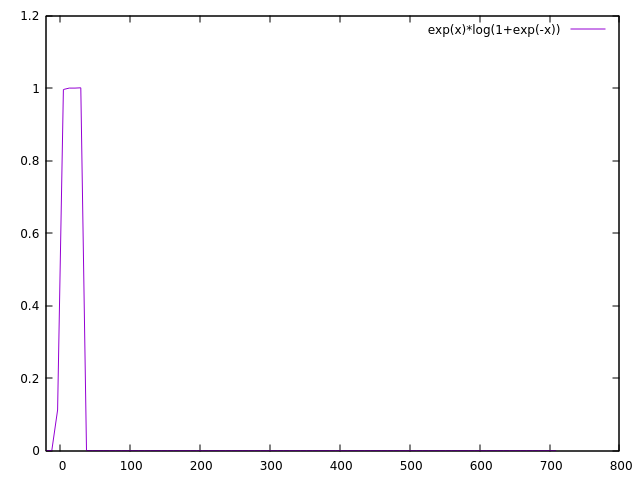
\includegraphics[width=0.5\textwidth]{zad2/GnuplotMax.png}} \hfill
			\subfloat[$x \in (31, 38)$ \label{fig:1b}]{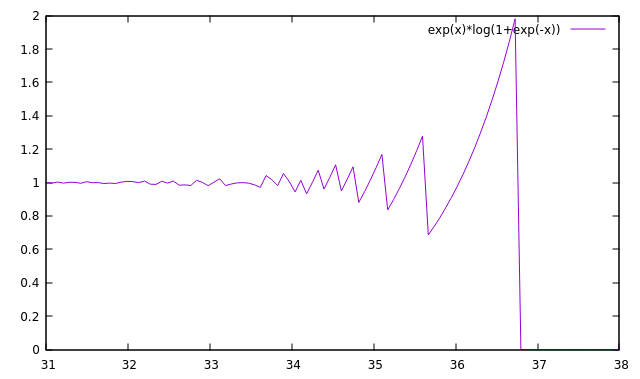
\includegraphics[width=0.5\textwidth]{zad2/GnuplotMin.png}}
  			\caption{Wykresy w \texttt{GNUPlot}.}
  			\label{fig:1}
		\end{figure}
		
		\begin{figure}[hpbt]
			\centering
			\subfloat[$x \in (-10, 800)$ \label{fig:2a}]{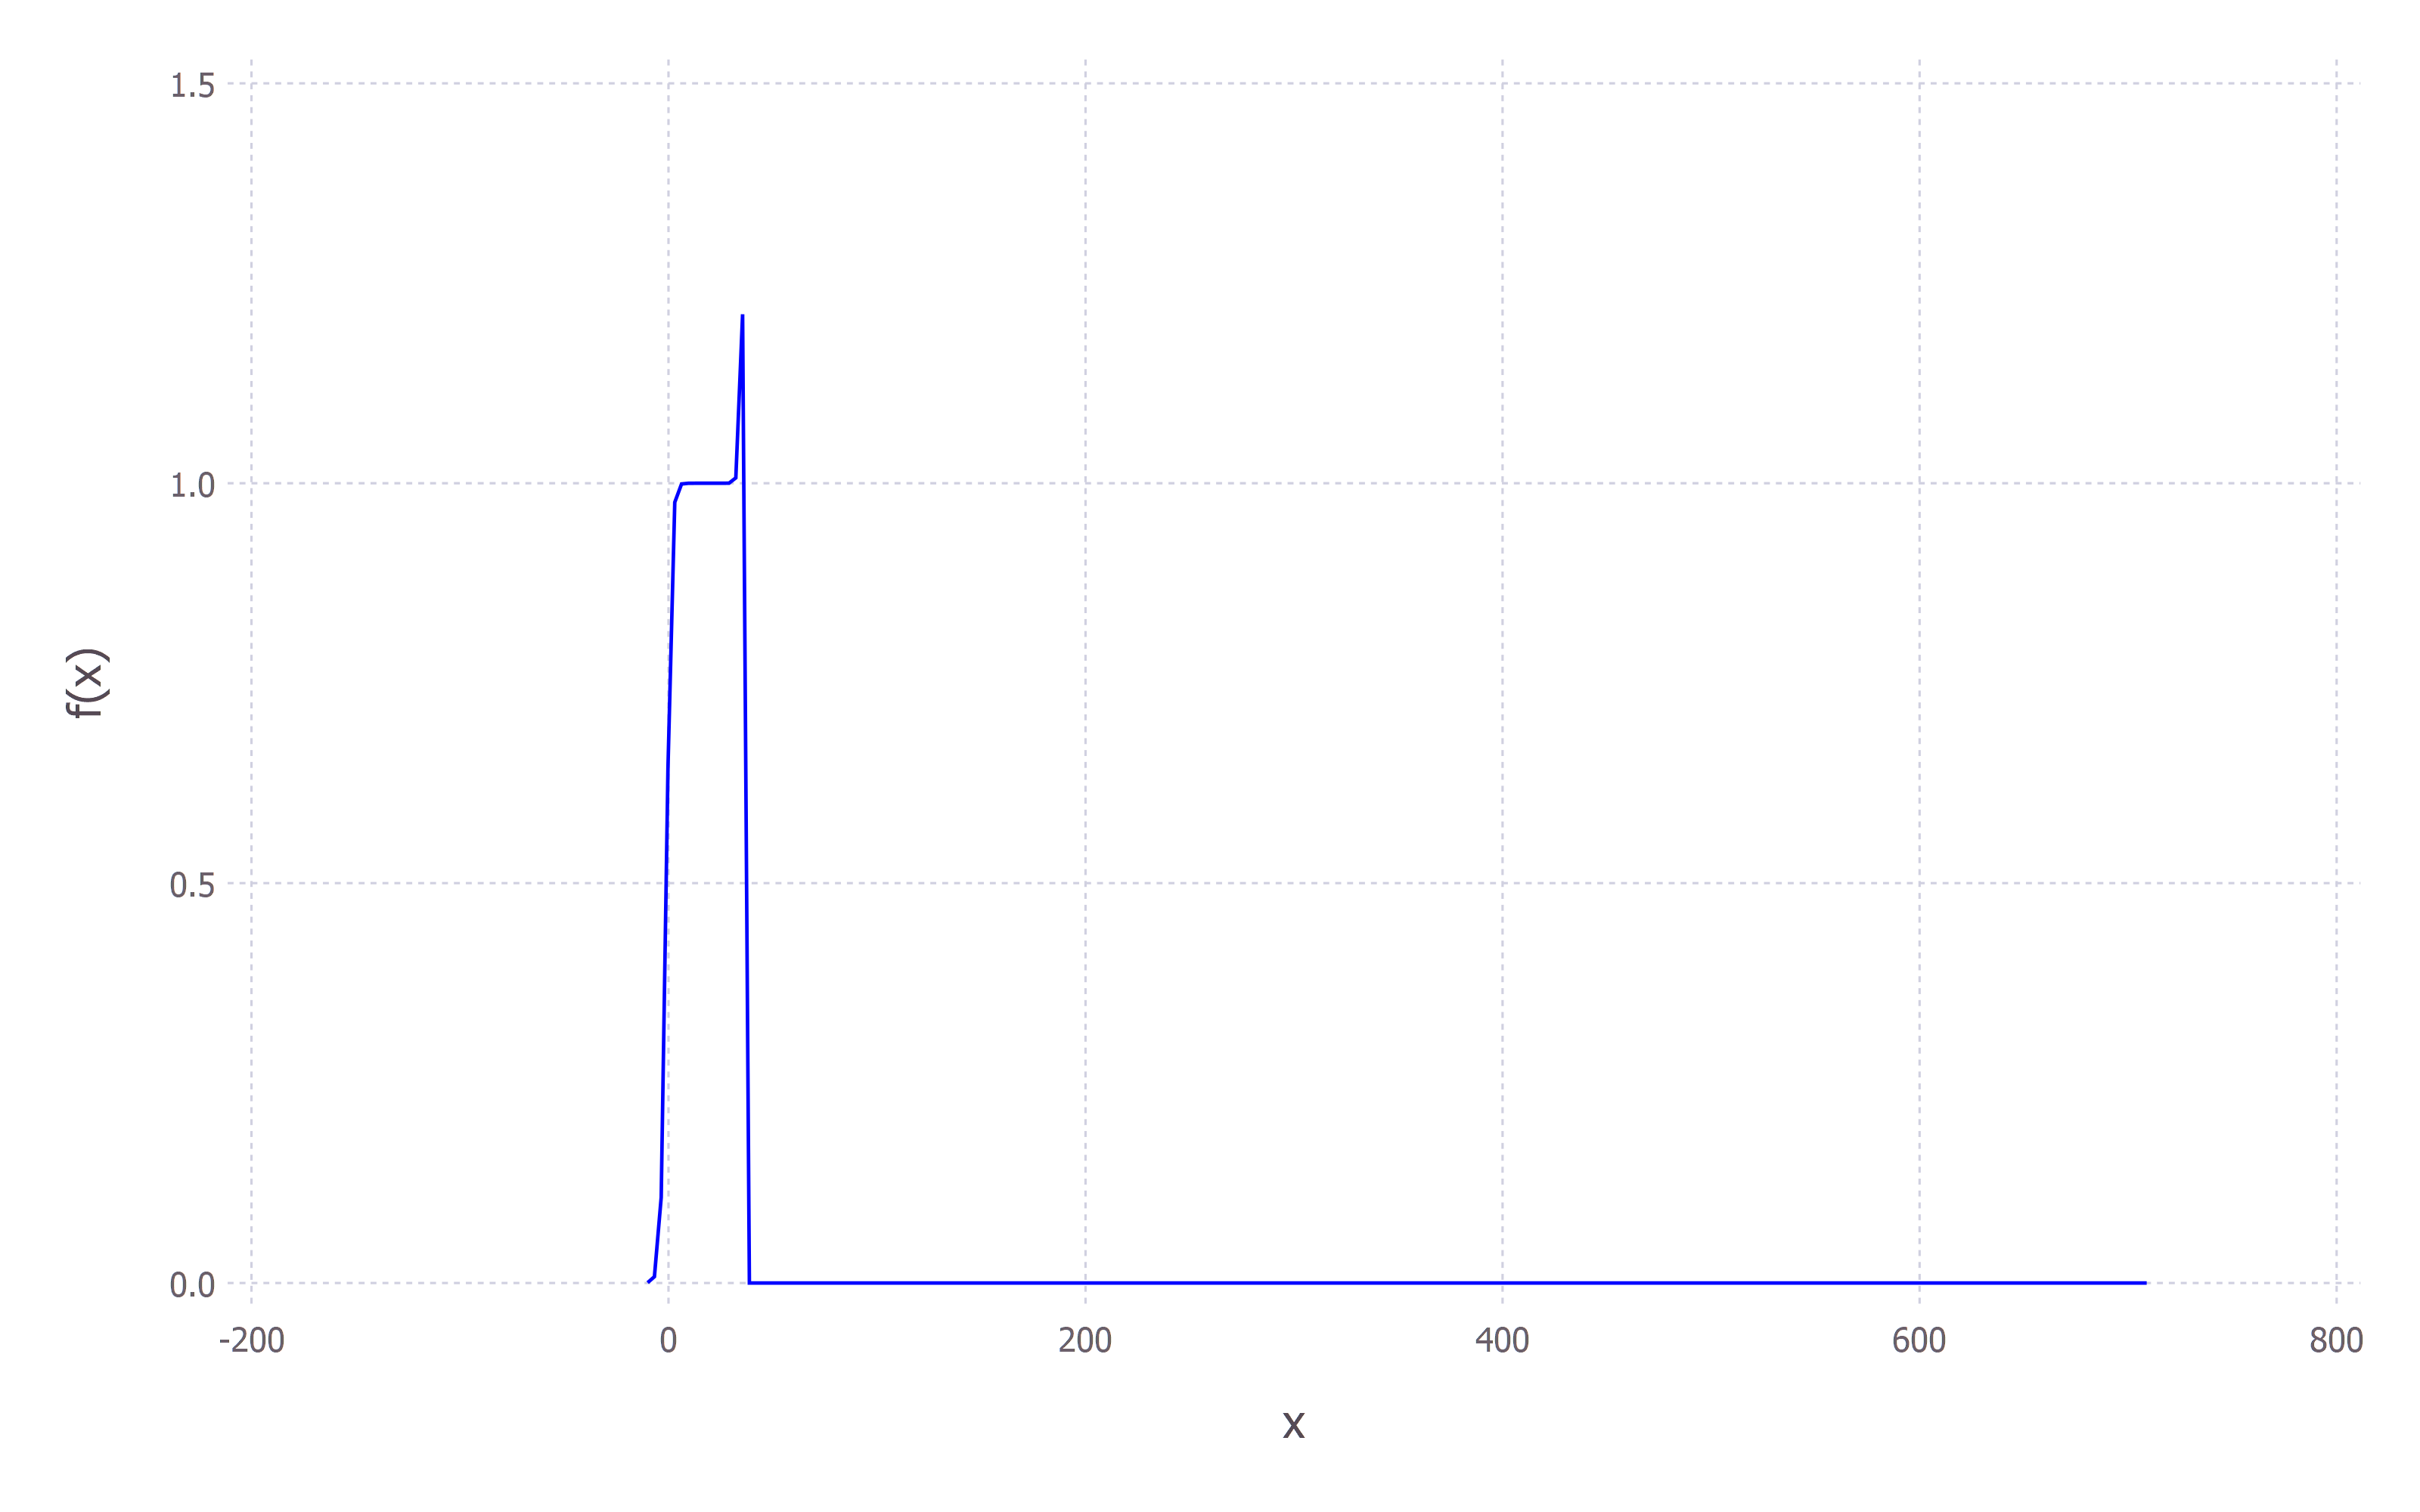
\includegraphics[width=0.5\textwidth]{zad2/plotGadfly1.png}} \hfill
			\subfloat[$x \in (31, 38)$ \label{fig:2b}]{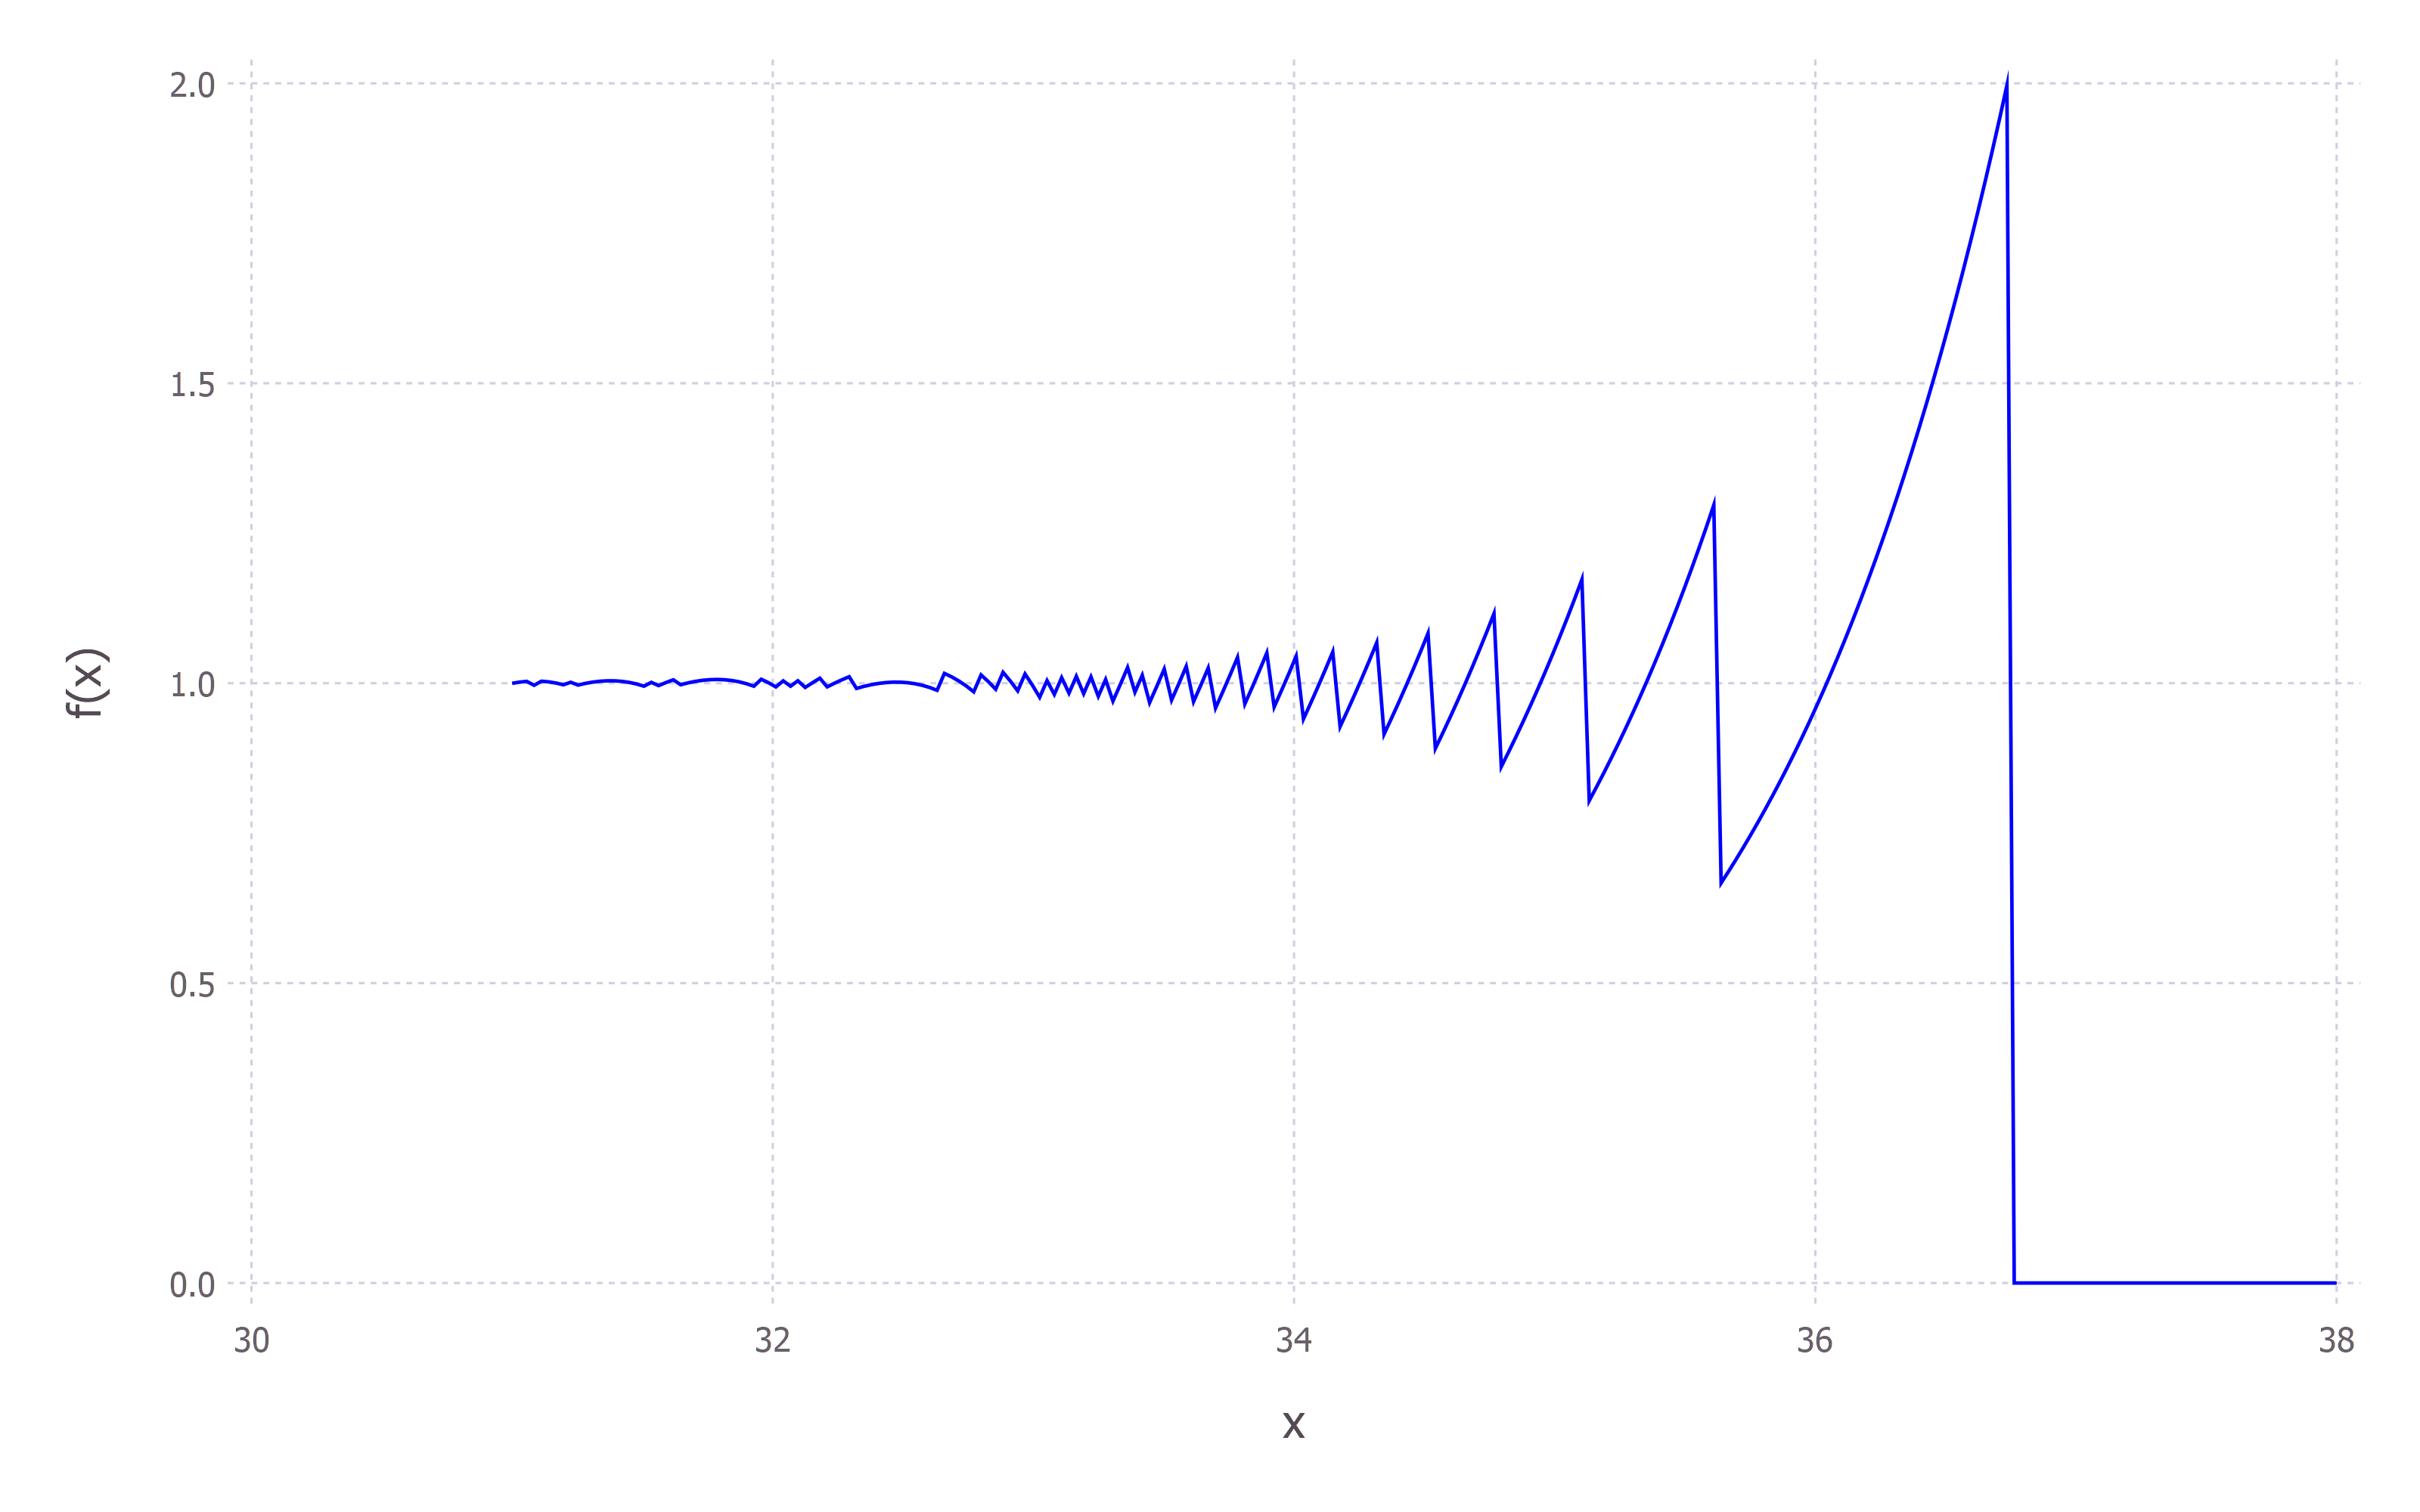
\includegraphics[width=0.5\textwidth]{zad2/plotGadfly2.png}}
  			\caption{Wykresy w \texttt{Gadfly}.}
  			\label{fig:2}
		\end{figure}
		
		\begin{figure}[hpbt]
			\centering
			\subfloat[$x \in (-10, 800)$ \label{fig:3a}]{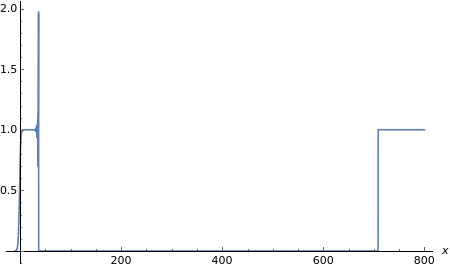
\includegraphics[width=0.5\textwidth]{zad2/Mathematica1.png}} \hfill
			\subfloat[$x \in (31, 38)$ \label{fig:3b}]{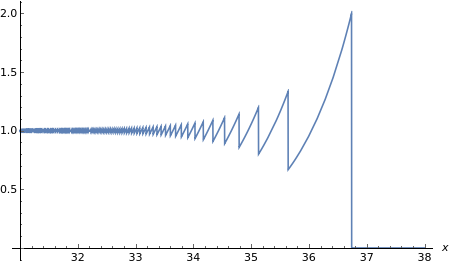
\includegraphics[width=0.5\textwidth]{zad2/Mathematica2.png}}
  			\caption{Wykresy w \texttt{Wolfram Alpha Cloud}.}
  			\label{fig:3}
		\end{figure}
		
	\subsection{Wnioski}
		Wykresy obrazują dość silną oscylację funkcji $f(x)$ dla pewnych argumentów $x > 31$ - można zauważyć przyjmowanie wartości większych niż 1 (niezgodność z wyliczoną granicą). Przyczyną takiego zachowania jest wykonywanie mnożenia bardzo małego logarytmu oraz dużej liczby $e(x)$, w efekcie czego generowane są znaczne błędy. Od pewnego $x$ funkcja osiąga stałą wartość równą 0. Powód stanowi bardzo już niewielka wartość $e(-x)$, co przekłada się na $\ln(1+e(-x))=\ln(1)=0$. Również ten problem jest źle uwarunkowany -- małe zmiany danych wpłynęły na duże odchylenia.
		
\section{Zadanie 3}
	\subsection{Opis problemu}
		Rozwiązanie układu równań liniowych $Ax = b$ dla danej macierzy współczynników $A \in {\rm I\!R^{n \times n}}$ i wektora prawych stron $b \in {\rm I\!R^n}$ za pomocą algorytmów: eliminacji Gaussa ($x=A/b$) oraz $x = A^{-1}b ~(x=inv(A)*b)$. 
		Macierz $A$ generowana jest w następujący sposób:
		\begin{enumerate}[(a)]
			\item $A = H_n$, gdzie $H_n$ jest macierzą Hilberta stopnia $n$;
			\item $A = R_n$, gdzie $R_n$ jest losową macierzą stopnia $n$ o zadanym wskaźniku uwarunkowania.
		\end{enumerate}
		Przeprowadzenie eksperymentów dla macierzy Hilberta $H_n$ z rosnącym stopniem $n > 1$ oraz dla macierzy losowej $R_n$, $n = 5, 10, 20$ z rosnącym wskaźnikiem uwarunkowania $c = 1, 10, 10^3, 10^7, 10^{12}, 10^{16}$, a także obliczenie błędów względnych.
	\subsection{Opis rozwiązania}
		W celu rozwiązania zadanego problemu utworzono w języku \texttt{Julia} funkcje konstruujące macierze (do wygenerowania macierzy Hilberta $n$--stopnia użyto \texttt{hilb($n$)}, zaś do losowej -- \texttt{matcond(c,$n$)} z dołączonych plików) i obliczające błędy względne dla dwóch podanych algorytmów.
	\subsection{Wyniki}
		Uzyskane rezultaty prezentują: Tabela \ref{table:2} oraz Tabela \ref{table:3}.
		\begin{table}[!h]
        	\centering
        	\footnotesize
			\sisetup{
				table-number-alignment = right,
				table-figures-integer = 4,
				table-figures-decimal = 17,
				table-figures-exponent = 3
			}
			\begin{tabular}{l|S|S|S} \toprule
				{$n$} & {\texttt{cond($n$)}} & {Eliminacja Gaussa} & {Odwrotność macierzy} \\ \midrule
				$1$ & 1.0 & 0.0 & 0.0 \\ 
	 			$2$ & 1.928147006790397e1 & 5.661048867003676e-16 & 1.4043333874306803e-15 \\
	 			$3$ & 5.240567775860644e2 & 8.022593772267726e-15 & 0.0 \\
	 			$4$ & 1.5513738738928138e4 & 3.861787750251888e-13 & 1.156679772130055e-13 \\
	 			$5$ & 4.7660725024172297e5 & 3.493384412947934e-13 & 1.3440842450589963e-11 \\ 
	 			$6$ & 1.4951058640747767e7 & 3.10690635252899e-10 & 2.1910589084611527e-10 \\
	 			$7$ & 4.753673563686169e8 & 1.4088888185246296e-8 & 1.2261030136487262e-8 \\
	 			$8$ & 1.5257575258900568e10 & 2.2563320836319543e-7 & 3.317498547889283e-7 \\ 
	 			$9$ & 4.9315447219360736e11 & 1.012295110413279e-5 & 1.0245032992812085e-5 \\
	 			$10$ & 1.602528535225018e13 & 1.658285788577287e-4 & 3.3373894670513554e-4 \\
	 			$11$ & 5.225191290892983e14 & 5.615377523997018e-3 & 7.4210143948519e-3 \\ 
	 			$12$ & 1.8025609727075732e16 & 1.8113059150336838e-1 & 2.0669418205518947e-1 \\
	 			$13$ & 1.1722023988382902e18 & 2.114212205460056 & 6.279218791835776e-1 \\ 
	 			$14$ & 4.892374250062484e17 & 1.1017472271829806e1 & 4.4152213858941764e1 \\
	 			$15$ & 1.1054293255916022e18 & 2.9364763338478763 & 4.600555824279512 \\
	 			$16$ & 4.3321097836601837e17 & 2.104258224602164 & 1.551741111529332e1 \\ 
	 			$17$ & 6.912464846448458e17 & 4.618693259670767 & 5.902966643537722 \\
	 			$18$ & 2.1386205784918858e18 & 5.8356203520913486 & 2.736241550426244e1\\ 
	 			$19$ & 5.7627595781335616e17 & 7.775664924181054 & 2.853711780136981e1 \\
	 			$20$ & 2.638328071362124e18  & 1.843691894440051e1 & 1.8274762664127028e1 \\ \bottomrule
	 		\end{tabular}
	 		\caption{Wskaźnik uwarunkowania oraz błędy względne dla macierzy Hilberta.}
			\label{table:2}
		\end{table}	
		
		
		\begin{table}[!h]
        	\centering
        	\footnotesize
			\sisetup{
				table-number-alignment = right,
				table-figures-integer = 4,
				table-figures-decimal = 17,
				table-figures-exponent = 3
			}
			\begin{tabular}{l|l|S|S} \toprule
				{$n$} & {$c$} & {Eliminacja Gaussa} & {Odwrotność macierzy} \\ \midrule
				$5$ & $1.0$ & 9.930136612989092e-17 & 1.7901808365247238e-16 \\ 
	 			$5$ & $10$ & 3.1401849173675503e-16 & 3.439900227959406e-16 \\
	 			$5$ & $10^3$ & 1.912137988767086e-14 & 2.383232787117382e-14 \\
	 			$5$ & $10^7$ & 3.3981049802510793e-10 & 3.389065765777984e-10 \\
	 			$5$ & $10^{12}$ & 7.4425034121248226e-6 & 6.716467613853077e-6 \\ 
	 			$5$ & $10^{16}$ & 2.5544448905136063e-1 & 1.767766952966369e-1 \\
	 			$10$ & $1$ & 3.7649494539356106e-16 & 2.673771110915334e-16 \\
	 			$10$ & $10$ & 3.8459253727671276e-16 & 3.255813018879823e-16 \\ 
	 			$10$ & $10^3$  & 1.3274015170704733e-14 & 1.3316753789632195e-14 \\
	 			$10$ & $10^7$ & 2.1562417902366395e-10 & 1.9095750411884216e-10 \\
	 			$10$ & $10^{12}$ & 2.3059687094933623e-5 & 1.899703918150136e-5 \\ 
	 			$10$ & $10^{16}$ & 1.657892355632386e-2 & 4.0042783982919855e-2 \\
	 			$20$ & $1$ & 5.032874986385111e-16 & 5.135906591666907e-16 \\ 
	 			$20$ & $10$ & 3.6988925808851116e-16 & 3.1791949213824894e-16 \\
	 			$20$ & $10^3$ & 2.0770979171517435e-14 & 1.903687736627341e-14 \\
	 			$20$ & $10^7$ & 2.6499281008781586e-10 & 2.1892654001923237e-10 \\ 
	 			$20$ & $10^{12}$ & 4.575827403624591e-5 & 4.661848415190589e-5 \\
	 			$20$ & $10^{16}$  & 7.272214577202413e-2 & 6.41115326598508e-2 \\ \bottomrule
	 		\end{tabular}
	 		\caption{Wskaźnik uwarunkowania oraz błędy względne dla macierzy losowej.}
			\label{table:3}
		\end{table}	
	\subsection{Wnioski}
		W przypadku macierzy Hilberta błąd rośnie wraz ze zwiększającą się wartością \texttt{cond} (co bezpośrednio związane jest z rosnącym stopniem). Błędy te są jednak większe dla algorytmu odwrotności macierzy (nie jest on zalecany z numerycznego punktu widzenia).	Z kolei dla macierzy generowanej w sposób losowy ewidentnie występuje wzrost błędów w miarę zwiększania się stopnia oraz wskaźnika uwarunkowania. Prowadzi to do konkluzji, iż wykonywanie obliczeń na macierzach o dużym wskaźniku uwarunkowania doprowadza do generowania dużych błędów obliczeniowych. Można by rzec, iż "złośliwość" macierzy jest wprost proporcjonalna do wskaźnika uwarunkowania, co prowadzi do wniosku, iż zadanie to jest źle uwarunkowane.
\section{Zadanie 4}
	\subsection{Opis problemu}
		Przeprowadzenie eksperymentu obliczania zer wielomianu Wilkinsona, zapisanego pod dwiema następującymi postaciami:
		$$P(x) = x^{20}-210x^{19}+20615x^{18} \dots $$
		$$p(x) = (x-20)(x-19)(x-18)\dots (x-2)(x-1)$$
		oraz określenie błędu bezwzględnego wartości tego wielomianu dla otrzymanych pierwiastków.
		Następnie powtórzenie testu dla współczynnika przy $x^{19}$ zmienionego na $-210-2^{-23}$.
	\subsection{Opis rozwiązania}
		Rozwiązanie zadania przygotowano w języku \texttt{Julia} z użyciem trzech funkcji dostępnych w pakiecie \texttt{Polynomials}. Przebiega ono zgodnie z poniższymi krokami:
		\begin{enumerate}[1.]
			\item Utworzenie wielomianu na podstawie podanych współczynników w postaci kanonicznej (funkcja \texttt{Poly}), a także iloczynowej (funkcja \texttt{poly});
			\item Obliczenie pierwiastków wielomianu $z_k, ~ 1 \le k \le 20$ przy użyciu funkcji \texttt{roots};
			\item Prezentacja błędu bezwzględnego obu postaci wielomianu oraz miejsc zerowych.
		\end{enumerate}
	\subsection{Wyniki}
		Otrzymane wyniki zaprezentowano w Tabelach \ref{table:4} oraz \ref{table:5}.	
	
		\begin{table}[!h]
        	\centering
        	\footnotesize
			\sisetup{
				table-number-alignment = right,
				table-figures-integer = 3,
				table-figures-decimal = 16,
				table-figures-exponent=2
			}
			
			\begin{tabular}{l|S|S|S} \toprule
				{k} & {$|P(z_k)|$} & {$|p(z_k)|$} & {$|z_k-k|$} \\ \midrule
				$1$ & 2.2016e4 & 2.2016e4 & 1.7530421558831222e-13 \\ 
	 			$2$ & 1.11104e5 & 1.11104e5 & 1.8059331807762646e-11 \\
	 			$3$ & 2.33472e5 & 2.33472e5 & 1.301203589321176e-10 \\
	 			$4$ & 3.204096e6 & 3.204096e6 & 1.9510343118867013e-8 \\
	 			$5$ & 1.1813888e7 & 1.1813888e7 & 2.7114605316569396e-7 \\ 
	 			$6$ & 1.39264e7 & 1.39264e7 & 3.6291786109643454e-7 \\
	 			$7$ & 1.32373504e8 & 1.32373504e8 & 2.1406434954407416e-5 \\
	 			$8$ & 4.73758208e8 & 4.73758208e8 & 2.4147412876196483e-4 \\ 
	 			$9$ & 1.653683712e9 & 1.653683712e9 & 1.4020327864088244e-3 \\
	 			$10$ & 8.700433408e9	 & 8.700433408e9	 & 5.402181223315594e-3 \\
	 			$11$ & 1.7547646464e10 & 1.7547646464e10 & 1.4432632050114691e-2 \\ 
	 			$12$ & 5.0825762816e10 & 5.0825762816e10 & 2.990002384475332e-2 \\
	 			$13$ & 9.3423894528e10 & 9.3423894528e10 & 4.396429964597992e-2 \\ 
	 			$14$ & 2.41390764032e11 & 2.41390764032e11 & 5.062781545541739e-2 \\
	 			$15$ & 3.71354137088e11 & 3.71354137088e11 & 4.358785452156155e-2 \\
	 			$16$ & 1.139728016896e12 & 1.139728016896e12 & 2.6199925603251017e-2 \\ 
	 			$17$ & 1.191399366656e12 & 1.191399366656e12 & 1.1769125575376904e-2 \\
	 			$18$ & 2.064536443392e12 & 2.064536443392e12 & 3.3212325988323244e-3 \\ 
	 			$19$ & 4.078909789184e12 & 4.078909789184e12 & 5.534781953926426e-4 \\
	 			$20$ & 6.50945294848e12 & 6.50945294848e12 & 3.82874895308305e-5 \\ \bottomrule
	 		\end{tabular}
	 		\caption{Błędy bezwzględne uzyskanych pierwiastków wielomianu Wilkinsona.}
			\label{table:4}
		\end{table}	
		
		\begin{table}[!h]
        	\centering
        	\footnotesize
			\sisetup{
				table-number-alignment = right,
				table-figures-integer = 2,
				table-figures-decimal = 16,
				table-figures-exponent=2
			}
					
			\begin{tabular}{l|l|S|S|S} \toprule
				{k} & {$z_k$} & {$|P(z_k)|$} & {$|z_k-k|$} \\ \midrule
				$1$ & $0.9999999999998185 + 0.0im$ & 2.3040e4 & 1.815214645262131e-13 \\ 
	 			$2$ & $2.0000000000367115 + 0.0im$ & 2.26304e5 & 3.6711522710675126e-11 \\
	 			$3$ & $2.9999999982108 + 0.0im$ & 1.020416e6 & 1.7891998993491143e-9 \\
	 			$4$ & $4.000000046165133 + 0.0im$ & 5.408768e6 & 4.6165133049669294e-8 \\
	 			$5$ & $4.999999028612442 + 0.0im$ & 2.4512e7 & 9.71387557946457e-7 \\ 
	 			$6$ & $6.000019095243171 + 0.0im$ & 1.18212096e8 & 1.909524317067479e-5 \\
	 			$7$ & $6.999593471115021 + 0.0im$ & 4.35741184e8 & 4.0652888497927364e-4 \\
	 			$8$ & $8.007845735396307 + 0.0im$ & 1.326422528e9 & 7.845735396307063e-3 \\ 
	 			$9$ & $8.91577894554576 + 0.0im$ & 2.641426944e9 & 8.422105445423966e-2 \\
	 			$10$ & $10.095898499560946 - 0.6443373996274354im$ & 3.933353845712834e9 & 6.514347294830742e-1 \\
	 			$11$ & $10.095898499560946 + 0.6443373996274354im$ & 3.933353845712834e9 & 1.1102117850458961 \\ 
	 			$12$ & $11.793856811906817 - 1.6517914101583042im$ & 5.607254943502496e10 & 1.6646050212197427 \\
	 			$13$ & $11.793856811906817 + 1.6517914101583042im$ & 5.607254943502496e10 & 2.0452863498435483 \\ 	 			
	 			$14$ & $13.99219600562902 - 2.5185303274174613im$ & 7.277997935632854e11 & 2.518542418235128 \\	 			
	 			$15$ & $13.99219600562902 + 2.5185303274174613im$ & 7.277997935632854e11 & 2.712685735796096 \\
	 			$16$ & $16.73061534277457 - 2.8125332877614704im$ & 9.452080179531715e12 & 2.905880636547886 \\ 
	 			$17$ & $16.73061534277457 + 2.8125332877614704im$ & 9.452080179531715e12 & 2.825404676911753 \\
	 			$18$ & $19.50237924554758 - 1.9403001967481368im$ & 6.223348199767701e13 & 2.4539576709782454 \\ 
	 			$19$ & $19.50237924554758 + 1.9403001967481368im$ & 6.223348199767701e13 & 2.004282854254313 \\
	 			$20$ & $20.84687198804629 + 0.0im$ & 1.48081940965376e14 & 8.468719880462885e-1 \\ \bottomrule
	 			
	 		\end{tabular}
	 		\caption{Błędy bezwzględne uzyskanych pierwiastków zmienionego wielomianu Wilkinsona.}
			\label{table:5}
		\end{table}	
	\subsection{Wnioski}
		Rzut oka pozwala dostrzec, że uzyskane wyniki różnią się znacznie od oczekiwanych. Miast zer, otrzymano liczby rzędu bilionów. Wyraźnie widoczny jest wzrost błędu wraz ze wzrostem wartości pierwiastka. Różnice początkowo nie są zbyt duże, jednak wraz z kolejnymi etapami obliczeń kumulują się, doprowadzając do tak diametralnych rozbieżności (np. dla $x_0 = 1, ~ z_0 = 1-\epsilon, ~|p(x_0)|=\epsilon \cdot 19!)$. Współczynniki wielomianu przekazywane jako argumenty funkcji \texttt{Poly(W)} nie mogą być dokładnie reprezentowane (dostępnych jest od 15 do 17 miejsc na cyfry znaczące systemu dziesiętnego), stąd wynikłe zaburzenia.
		Przebieg drugiego eksperymentu był analogiczny, poczyniono jednak nieznaczne zmiany w jednym ze współczynników danego wielomianu. W rezultacie otrzymano zauważalne różnice w błędach bezwzględnych obliczonych pierwiastków -- są zdecydowanie wyższe niż w przypadku niezmienionego wielomianu Wilkinsona. Dodatkowo istotnym spostrzeżeniem jest uzyskanie pierwiastków należących do liczb zespolonych -- część urojona pojawia się od $z_{10}$. Niewielkie zaburzenia wpłynęły znacząco na odkształcenie wyników, zatem zadanie to jest źle uwarunkowane.
\section{Zadanie 5}
	\subsection{Opis problemu}
		Przeprowadzenie dwóch eksperymentów przy wykorzystaniu następującego modelu wzrostu populacji: $$p_{n+1} := p_n + rp_n(1-p_n), \text{ dla } n = 1, 2, \dots,$$
		gdzie $r$ jest pewną stałą, $r(1-p_n)$ jest czynnikiem wzrostu populacji, a $p_0$ jest wielkością populacji stanowiącą procent maksymalnej wielkości populacji dla danego stanu środowiska.
		Testy przeprowadzić dla danych wejściowych we wskazanych arytmetykach:
		\begin{enumerate}[(a)]
			\item $p_0 = 0.01$, $r = 3$, $n = 40$ \{\texttt{Float32}\}
			\item $p_0 = 0.01$, $r = 3$, $n = 40$ \{\texttt{Float64}\}
			\item $p_0 = 0.01$, $r = 3$, $n = 40$, po 10 iteracjach zastosowanie obcięcia wyniku do trzeciego miejsca po przecinku \{\texttt{Float32}\}.
		\end{enumerate}
	\subsection{Opis rozwiązania}
		Rozwiązanie problemu zrealizowano w języku \texttt{Julia}. Utworzono dwie funkcje, które wykonują 40 iteracji, wyliczając wartość $p_n$, a następnie zapisują ją w tablicy (przy czym druga z funkcji po 10 przebiegach pętli dokonuje obcięcia wyniku). Algorytm pierwszej z nich przedstawiony został na poniższym listingu:
		
		\begin{algorithm}
			\begin{algorithmic}
				\State $A \gets [0,0,\dots,0]$
				\State $p\gets 0.01$
				\State $A[1] \gets p$
				\State $i \gets 1$
				\While {$i < n$}
					\State {$p \gets p + r*p*(1.0-p)$}
					\State $A[i+1] \gets p$
					\State $i \gets i+1$
				\EndWhile
				\State return $A$
			\end{algorithmic}
			\caption{}
		\end{algorithm}		
		
	\subsection{Wyniki}
		Uzyskane rezultaty dla przeprowadzonych eksperymentów zaprezentowano na Rysunku \ref{fig:4}.
		
		\begin{figure}[htbp]
			\centering
			\subfloat[1.][(a.) oraz (c.).]{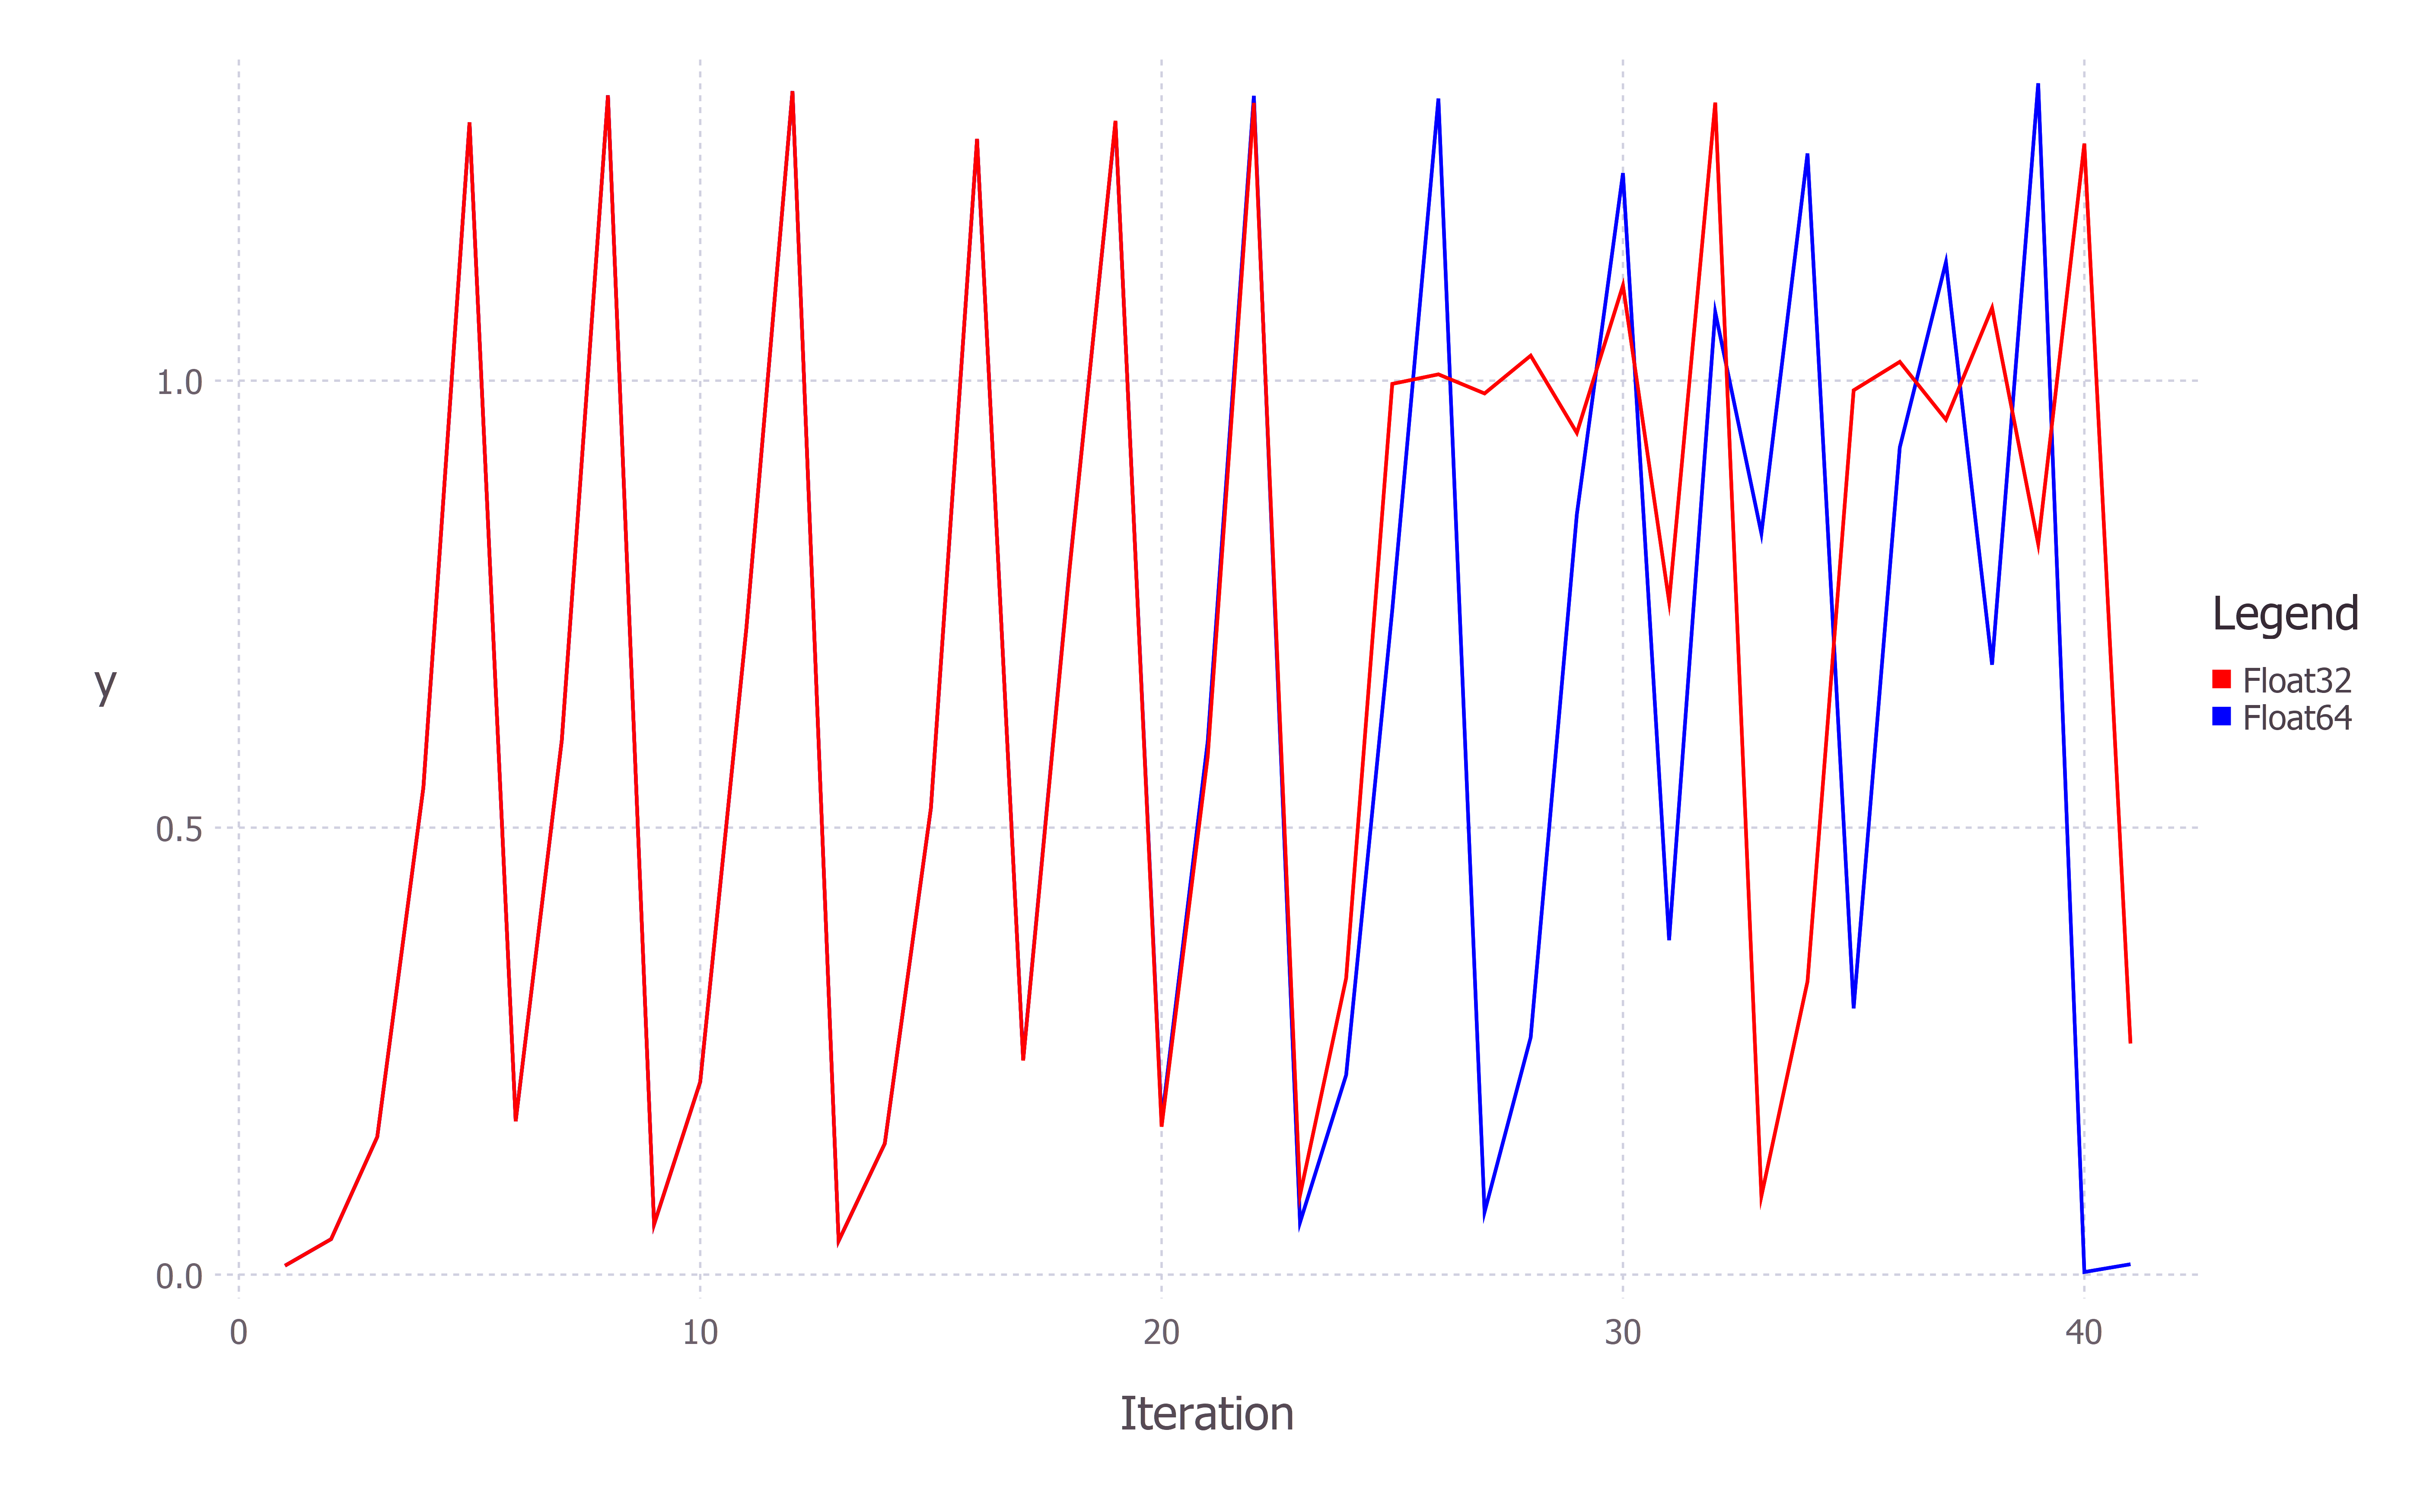
\includegraphics[width=0.5\textwidth]{zad5/plot1.png}} \hfill
			\subfloat[2.][(a.) oraz (b.).]{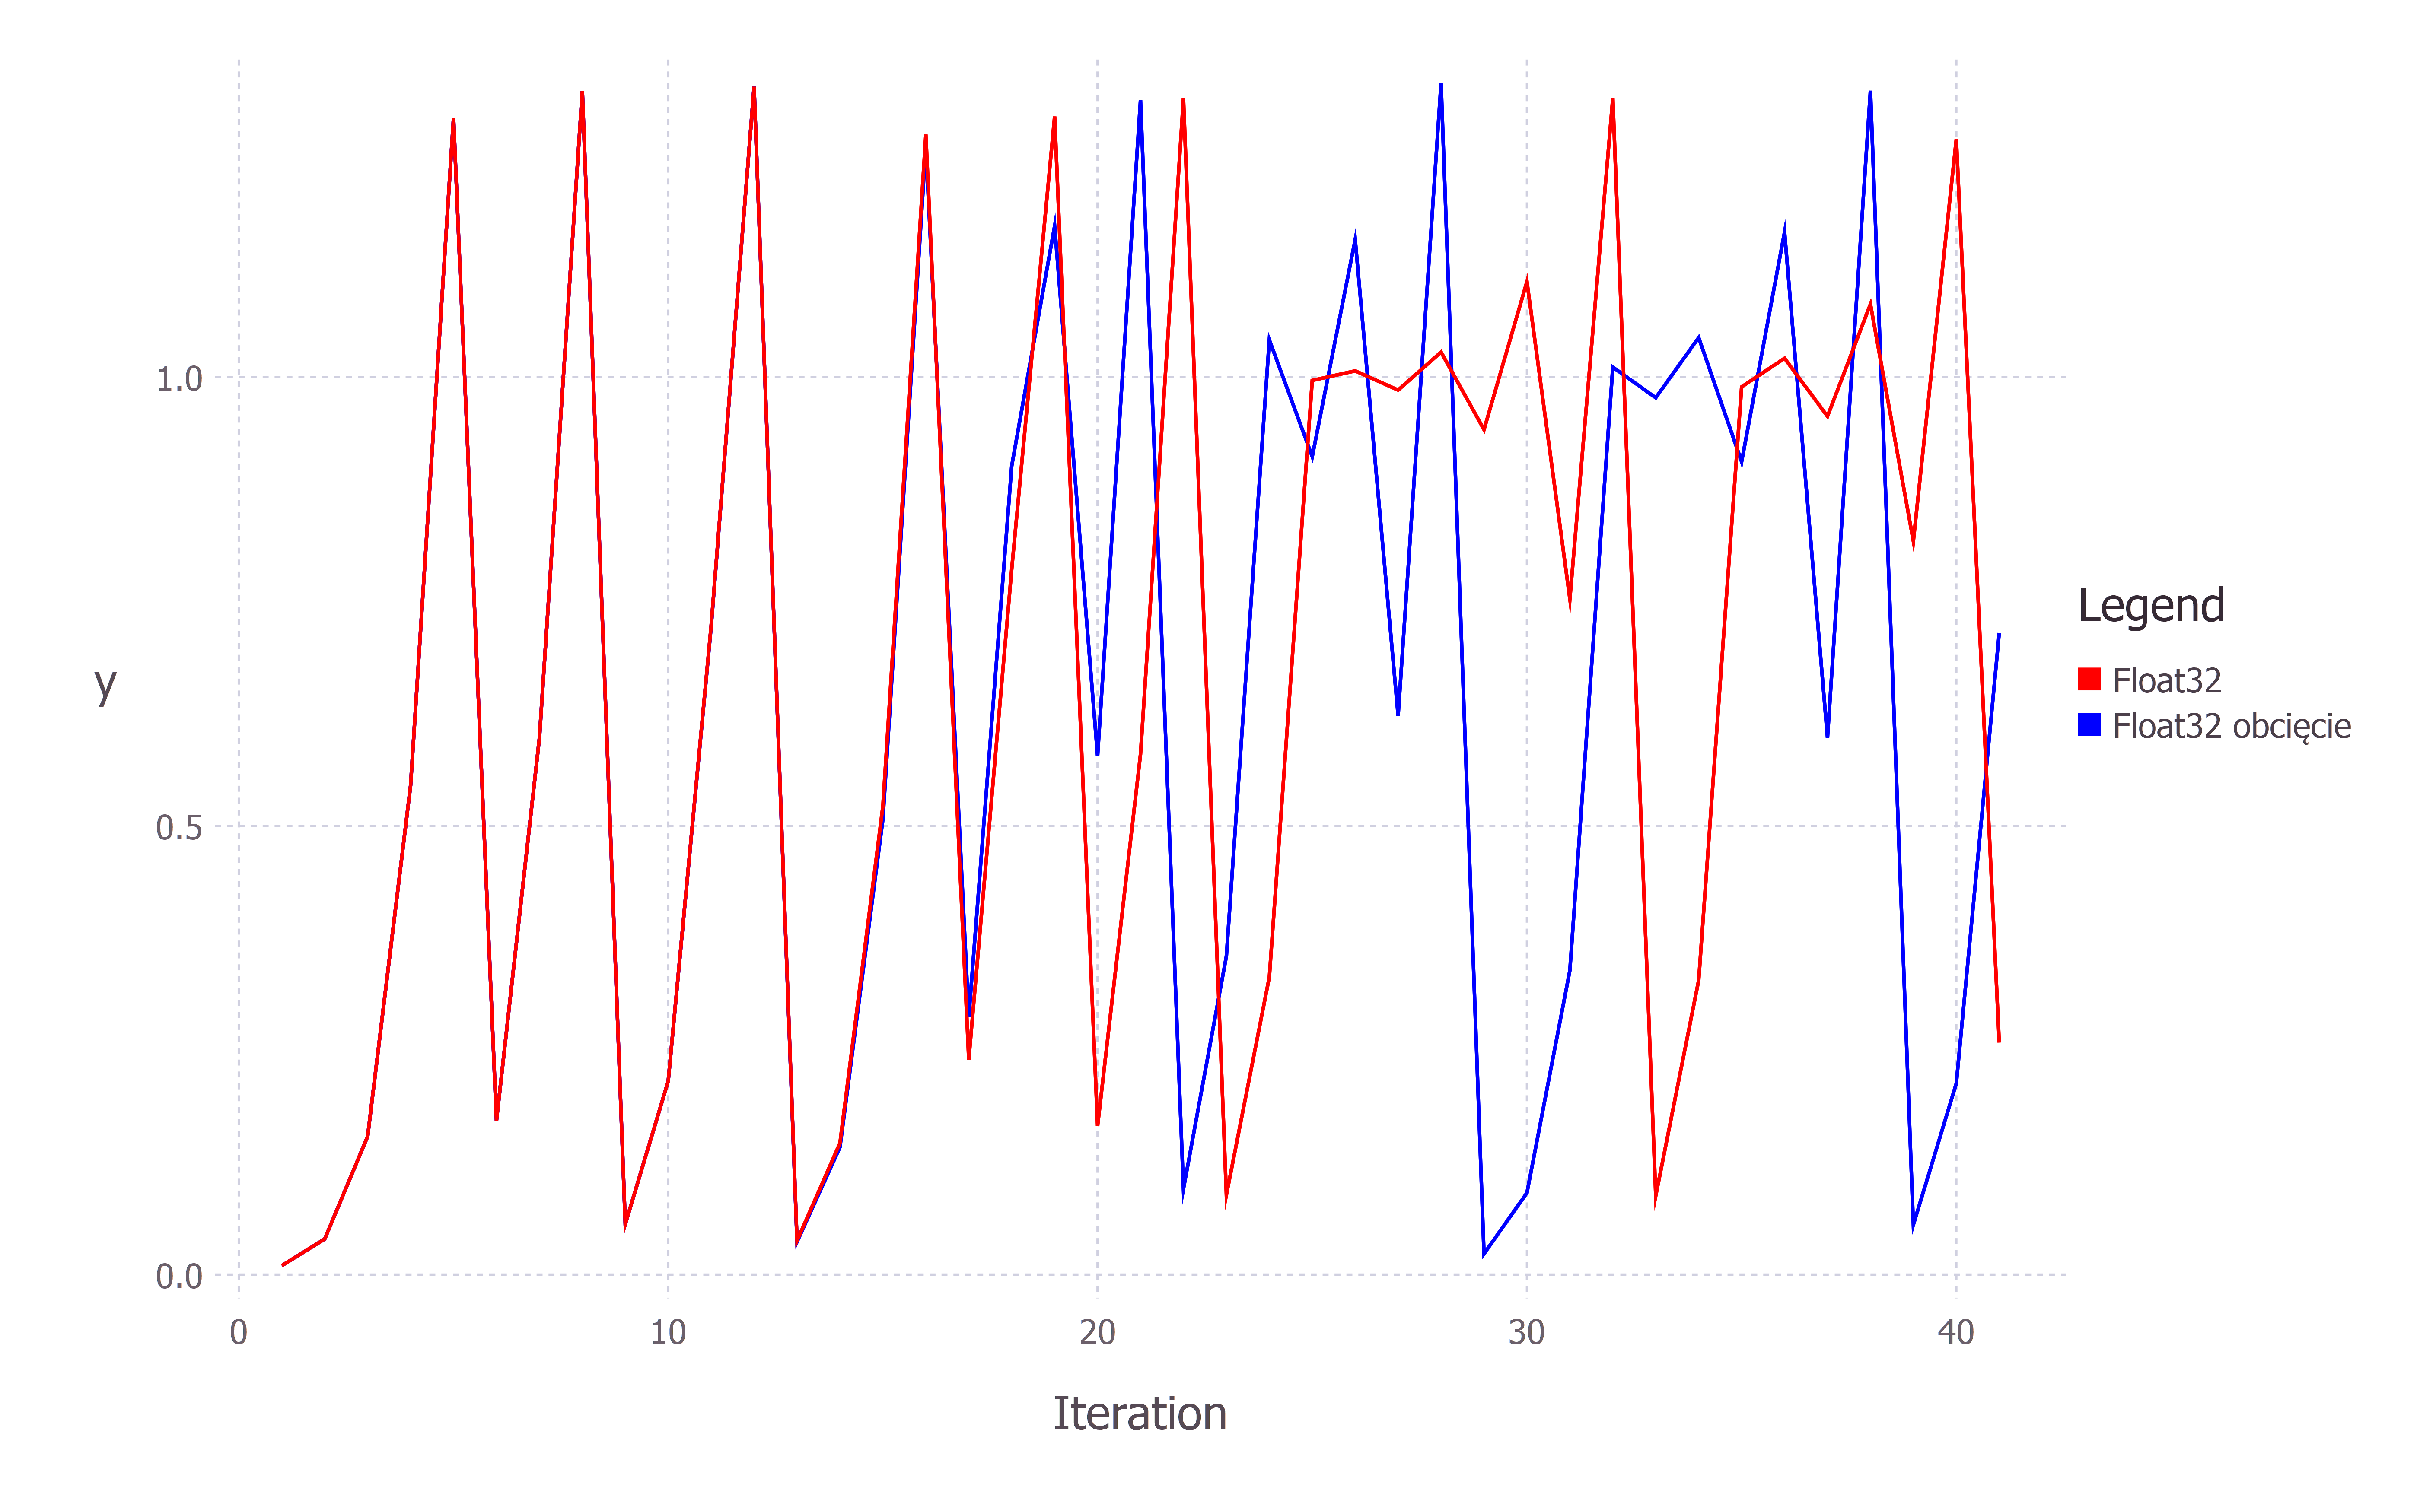
\includegraphics[width=0.5\textwidth]{zad5/plot2.png}}
  			\caption{Zestawienie wyników dla konkretnych danych}
  			\label{fig:4}
		\end{figure}		
		
	\subsection{Wnioski}
		W przypadku pierwszego eksperymentu doskonale można zaobserwować, jak, początkowo zdawałoby się znikomy, błąd staje się wraz z kolejnymi przebiegami tak duży, iż uzyskujemy niemal nową, oddzielną iterację (wynik zgodny jest co do części tysięcznej, czyli w każdej kolejnej iteracji pojawia się różnica pomiędzy rozwiązaniami). W przypadku arytmetyki \texttt{Float32} dostępnych jest tylko 6-9 cyfr znaczących, których, w miarę postępowania iteracji, potrzeba coraz więcej by móc zapisać prawidłowy wynik.

		Analiza drugiego wykresu pozwala dostrzec różnice w regularności przebiegu. Niższa precyzja arytmetyki \texttt{Float32} wpłynęła na stale powiększające się różnice, by osiągnąć swoistą kulminacyjną wartość równą $1.0$. Każda kolejna iteracja oscylowała w pobliżu właśnie tego wyniku.
		Ciekawym spostrzeżeniem jest fakt, iż dla \texttt{Float64} ma miejsce podobna sytuacja, jednak w znacznie dalszej iteracji. 
		
		Powyższe eksperymenty pozwalają dostrzec, że błąd obliczeniowy wyniku, przeniesiony jako wejście kolejnej operacji, potęguje powstały błąd. Jest to typowy przykład sprzężenia zwrotnego - procesu, w którym dane wyjściowe jednego problemu są wejściem kolejnych obliczeń. Zaskakującym jest natomiast fakt nieskorelowania, co wskazuje na istnienie chaosu w systemie czy też może zjawisko niemożności przewidzenia (zgodnie ze sformułowaniem Lorenza). W uniknięciu tego rodzaju sytuacji pomóc może zwiększenie precyzji obliczeń, choć jednak w daleko wybiegających symulacjach powstałe błędy mogą zniekształcić obliczenia w tak dużym stopniu, iż również te wyniki staną się dla badającego bezużyteczne. Biorąc pod uwagę powyższe rozważania, niemożliwym jest uniknięcie błędów zaokrągleń, które są w pewien sposób integralną częścią obliczeń w arytmetyce zmiennopozycyjnej. Taki efekt będzie miał miejsce na każdym urządzeniu, niezależnie od jego mocy obliczeniowej. Stąd prosty wniosek -- zadanie jest źle uwarunkowane.
		
\section{Zadanie 6}
	\subsection{Opis problemu}
		Przeprowadzenie eksperymentów w języku \texttt{Julia} w arytmetyce \texttt{Float64} dla następującego równania rekurencyjnego:
		$$x_{n+1} := x^{2}_{n} + c \text{ dla } n = 0, 1, \dots,$$
		gdzie $c$ jest pewną stałą, dla danych wejściowych:
		\begin{enumerate}
			\item $c = -2$ i $x_0 = 1$;
			\item $c = -2$ i $x_0 = 2$;
			\item $c = -2$ i $x_0 = 1.99999999999999$;
			\item $c = -1$ i $x_0 = 1$;
			\item $c = -1$ i $x_0 = -1$;
			\item $c = -1$ i $x_0 = 0.75$;
			\item $c = -1$ i $x_0 = 0.25$;
		\end{enumerate}
		oraz ilości iteracji $n = 40$.
	\subsection{Opis rozwiązania}
		W języku \texttt{Julia} skonstruowano funkcję \texttt{calculate($x_0$,$c$)}, która wykonuje $n$ iteracji, obliczając aktualną wartość zgodnie z podanym w zadaniu wzorem. Uzyskane w ten sposób rozwiązania przechowywane są w tablicy, a następnie generowane są odpowiednie wykresy.
		
	\subsection{Wyniki}
		Tabela \ref{table:6} przedstawia wyniki eksperymentów uzyskane dla kolejnych iteracji $1 \le k \le n$.	
	
		\begin{table}[h]
	        \centering
	        \scriptsize
			\begin{tabular}{c
				|S[
		        table-number-alignment = right,
				table-figures-integer  = 2,
				table-figures-decimal = 1
				]
				|S[
		        table-number-alignment = right,
				table-figures-integer  = 2,
				table-figures-decimal = 1
				]
				|S[
		        table-number-alignment = right,
				table-figures-integer  = 2,
				table-figures-decimal = 16
				]
				|S[
		        table-number-alignment = right,
				table-figures-integer  = 2,
				table-figures-decimal = 1
				]
				|S[
		        table-number-alignment = right,
				table-figures-integer  = 2,
				table-figures-decimal = 1
				]
				|S[
		        table-number-alignment = right,
				table-figures-integer  = 2,
				table-figures-decimal = 16,
				table-figures-exponent=2
				]
				|S[
		        table-number-alignment = right,
				table-figures-integer  = 2,
				table-figures-decimal = 15,
				table-figures-exponent=2
				]}
				%\toprule
				\multirow{2}{*}{$k$} & \multicolumn{7}{c}{Eksperyment}  \\ \cline{2-8}
				&{$1.$}&{$2.$}&{$3.$}&{$4.$}&{$5.$}&{$6.$}&{$7.$} \\ \hline
				1&-1.0&2.0&1.99999999999996&0.0&0.0&-0.4375&-0.9375 \\
				2&-1.0&2.0&1.9999999999998401&-1.0&-1.0&-0.80859375&-0.12109375 \\
				3&-1.0&2.0&1.9999999999993605&0.0&0.0&-0.3461761474609375&-0.9853363037109375 \\
				4&-1.0&2.0&1.999999999997442&-1.0&-1.0&-0.8801620749291033&-0.029112368589267135 \\
				5&-1.0&2.0&1.9999999999897682&0.0&0.0&-0.2253147218564956&-0.9991524699951226 \\
				6&-1.0&2.0&1.9999999999590727&-1.0&-1.0&-0.9492332761147301&-0.0016943417026455965 \\
				7&-1.0&2.0&1.999999999836291&0.0&0.0&-0.0989561875164966&-0.9999971292061947 \\
				8&-1.0&2.0&1.9999999993451638&-1.0&-1.0&-0.9902076729521999&-5.741579369278327e-6 \\
				9&-1.0&2.0&1.9999999973806553&0.0&0.0&-0.01948876442658909&-0.9999999999670343 \\
				10&-1.0&2.0&1.999999989522621&-1.0&-1.0&-0.999620188061125&-6.593148249578462e-11 \\
				11&-1.0&2.0&1.9999999580904841&0.0&0.0&-0.0007594796206411569&-1.0 \\
				12&-1.0&2.0&1.9999998323619383&-1.0&-1.0&-0.9999994231907058&0.0 \\
				13&-1.0&2.0&1.9999993294477814&0.0&0.0&-1.1536182557003727e-6&-1.0 \\
				14&-1.0&2.0&1.9999973177915749&-1.0&-1.0&-0.9999999999986692&0.0 \\
				15&-1.0&2.0&1.9999892711734937&0.0&0.0&-2.6616486792363503e-12&-1.0 \\
				16&-1.0&2.0&1.9999570848090826&-1.0&-1.0&-1.0&0.0 \\
				17&-1.0&2.0&1.999828341078044&0.0&0.0&0.0&-1.0 \\
				18&-1.0&2.0&1.9993133937789613&-1.0&-1.0&-1.0&0.0 \\
				19&-1.0&2.0&1.9972540465439481&0.0&0.0&0.0&-1.0 \\
				20&-1.0&2.0&1.9890237264361752&-1.0&-1.0&-1.0&0.0 \\
				21&-1.0&2.0&1.9562153843260486&0.0&0.0&0.0&-1.0 \\
				22&-1.0&2.0&1.82677862987391&-1.0&-1.0&-1.0&0.0 \\
				23&-1.0&2.0&1.3371201625639997&0.0&0.0&0.0&-1.0 \\
				24&-1.0&2.0&-0.21210967086482313&-1.0&-1.0&-1.0&0.0 \\
				25&-1.0&2.0&-1.9550094875256163&0.0&0.0&0.0&-1.0 \\
				26&-1.0&2.0&1.822062096315173&-1.0&-1.0&-1.0&0.0 \\
				27&-1.0&2.0&1.319910282828443&0.0&0.0&0.0&-1.0 \\
				28&-1.0&2.0&-0.2578368452837396&-1.0&-1.0&-1.0&0.0 \\
				29&-1.0&2.0&-1.9335201612141288&0.0&0.0&0.0&-1.0 \\
				30&-1.0&2.0&1.7385002138215109&-1.0&-1.0&-1.0&0.0 \\
				31&-1.0&2.0&1.0223829934574389&0.0&0.0&0.0&-1.0 \\
				32&-1.0&2.0&-0.9547330146890065&-1.0&-1.0&-1.0&0.0 \\
				33&-1.0&2.0&-1.0884848706628412&0.0&0.0&0.0&-1.0 \\
				34&-1.0&2.0&-0.8152006863380978&-1.0&-1.0&-1.0&0.0 \\
				35&-1.0&2.0&-1.3354478409938944&0.0&0.0&0.0&-1.0 \\
				36&-1.0&2.0&-0.21657906398474625&-1.0&-1.0&-1.0&0.0 \\
				37&-1.0&2.0&-1.953093509043491&0.0&0.0&0.0&-1.0 \\
				38&-1.0&2.0&1.8145742550678174&-1.0&-1.0&-1.0&0.0 \\
				39&-1.0&2.0&1.2926797271549244&0.0&0.0&0.0&-1.0 \\
				40&-1.0&2.0&-0.3289791230026702&-1.0&-1.0&-1.0&0.0 \\
			\end{tabular}
			\caption{Iteracje w arytmetykach \texttt{Float32} oraz \texttt{Float64}}
			\label{table:6}
		\end{table}	

	\subsection{Wnioski}
%		W przypadku pierwszego oraz drugiego eksperymentu uzyskane wyniki są stabilne.
%		Trzecie doświadczenie jednak pokazuje, jak niewielkie odchylenie ($x_0 = 1.99999999999999$) niesie ze sobą w rezultacie zachowanie nieuporządkowane. Do takich wniosków prowadzić mogło Zadanie 5, jednak tutaj sytuacja jest bardziej złożona.
%		Dalsze eksperymenty poczyniono na dość radykalnie zmienionych danych blablabla...
%		Układ, powtarzając za autorem książki "Granice chaosu. Fraktale", jest w stanie idealnie stabilnym.
		
		Wizualizacje obu funkcji (Rysunek \ref{fig:5}, \ref{fig:6}) pozwalają wyciągnąć kolejne wnioski.
		\begin{figure}[htbp]
			\centering
			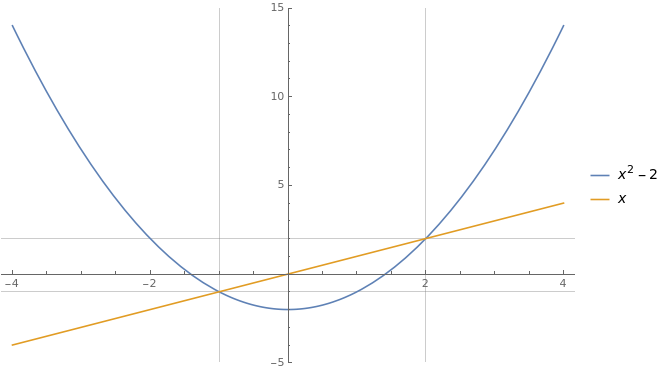
\includegraphics[width=0.8\textwidth]{zad6/Myplot1.png}
  			\caption{$\phi=x^2-2$, $f(x)=x$}
  			\label{fig:5}
		\end{figure}	
		
		\begin{enumerate}[1.]
			\item $x_0 = 1 ~\Rightarrow~ \phi(x)$ zbieżna do $-1$.
			\item $x_0 = 2 ~\Rightarrow~ \phi(x)$ zbieżna do $2$.
			\item $x_0 = 1.99999999999999 ~\Rightarrow~ \phi(x)$ rozbieżna.
		\end{enumerate}
		
		\begin{figure}[htbp]
			\centering
			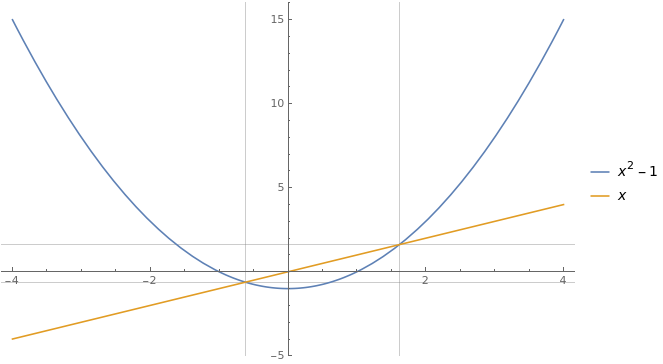
\includegraphics[width=0.8\textwidth]{zad6/Myplot2.png}
  			\caption{$\phi=x^2-1$, $f(x)=x$}
  			\label{fig:6}
		\end{figure}
		
		\begin{enumerate}[1.]
			\item $x_0 = 1 ~\Rightarrow$ podciąg wyrazów nieparzystych $\phi(x)$ zbieżny do $0$, zaś parzystych: $-1$.
			\item $x_0 = -1 ~\Rightarrow$ podciąg wyrazów nieparzystych $\phi(x)$ zbieżny do $0$, zaś parzystych: $-1$.
			\item $x_0 = 0.75 ~\Rightarrow$ podciąg wyrazów nieparzystych $\phi(x)$ (od pewnego $x$) zbieżny do $0$, zaś parzystych: $-1$.
			\item $x_0 = 0.25 ~\Rightarrow$ podciąg wyrazów nieparzystych $\phi(x)$ (od pewnego $x$) zbieżny do $0$, zaś parzystych: $-1$.
		\end{enumerate}
\end{document}

			
%		\begin{figure}[htbp]
%			\centering
%			\subfloat[1.][Plot3]{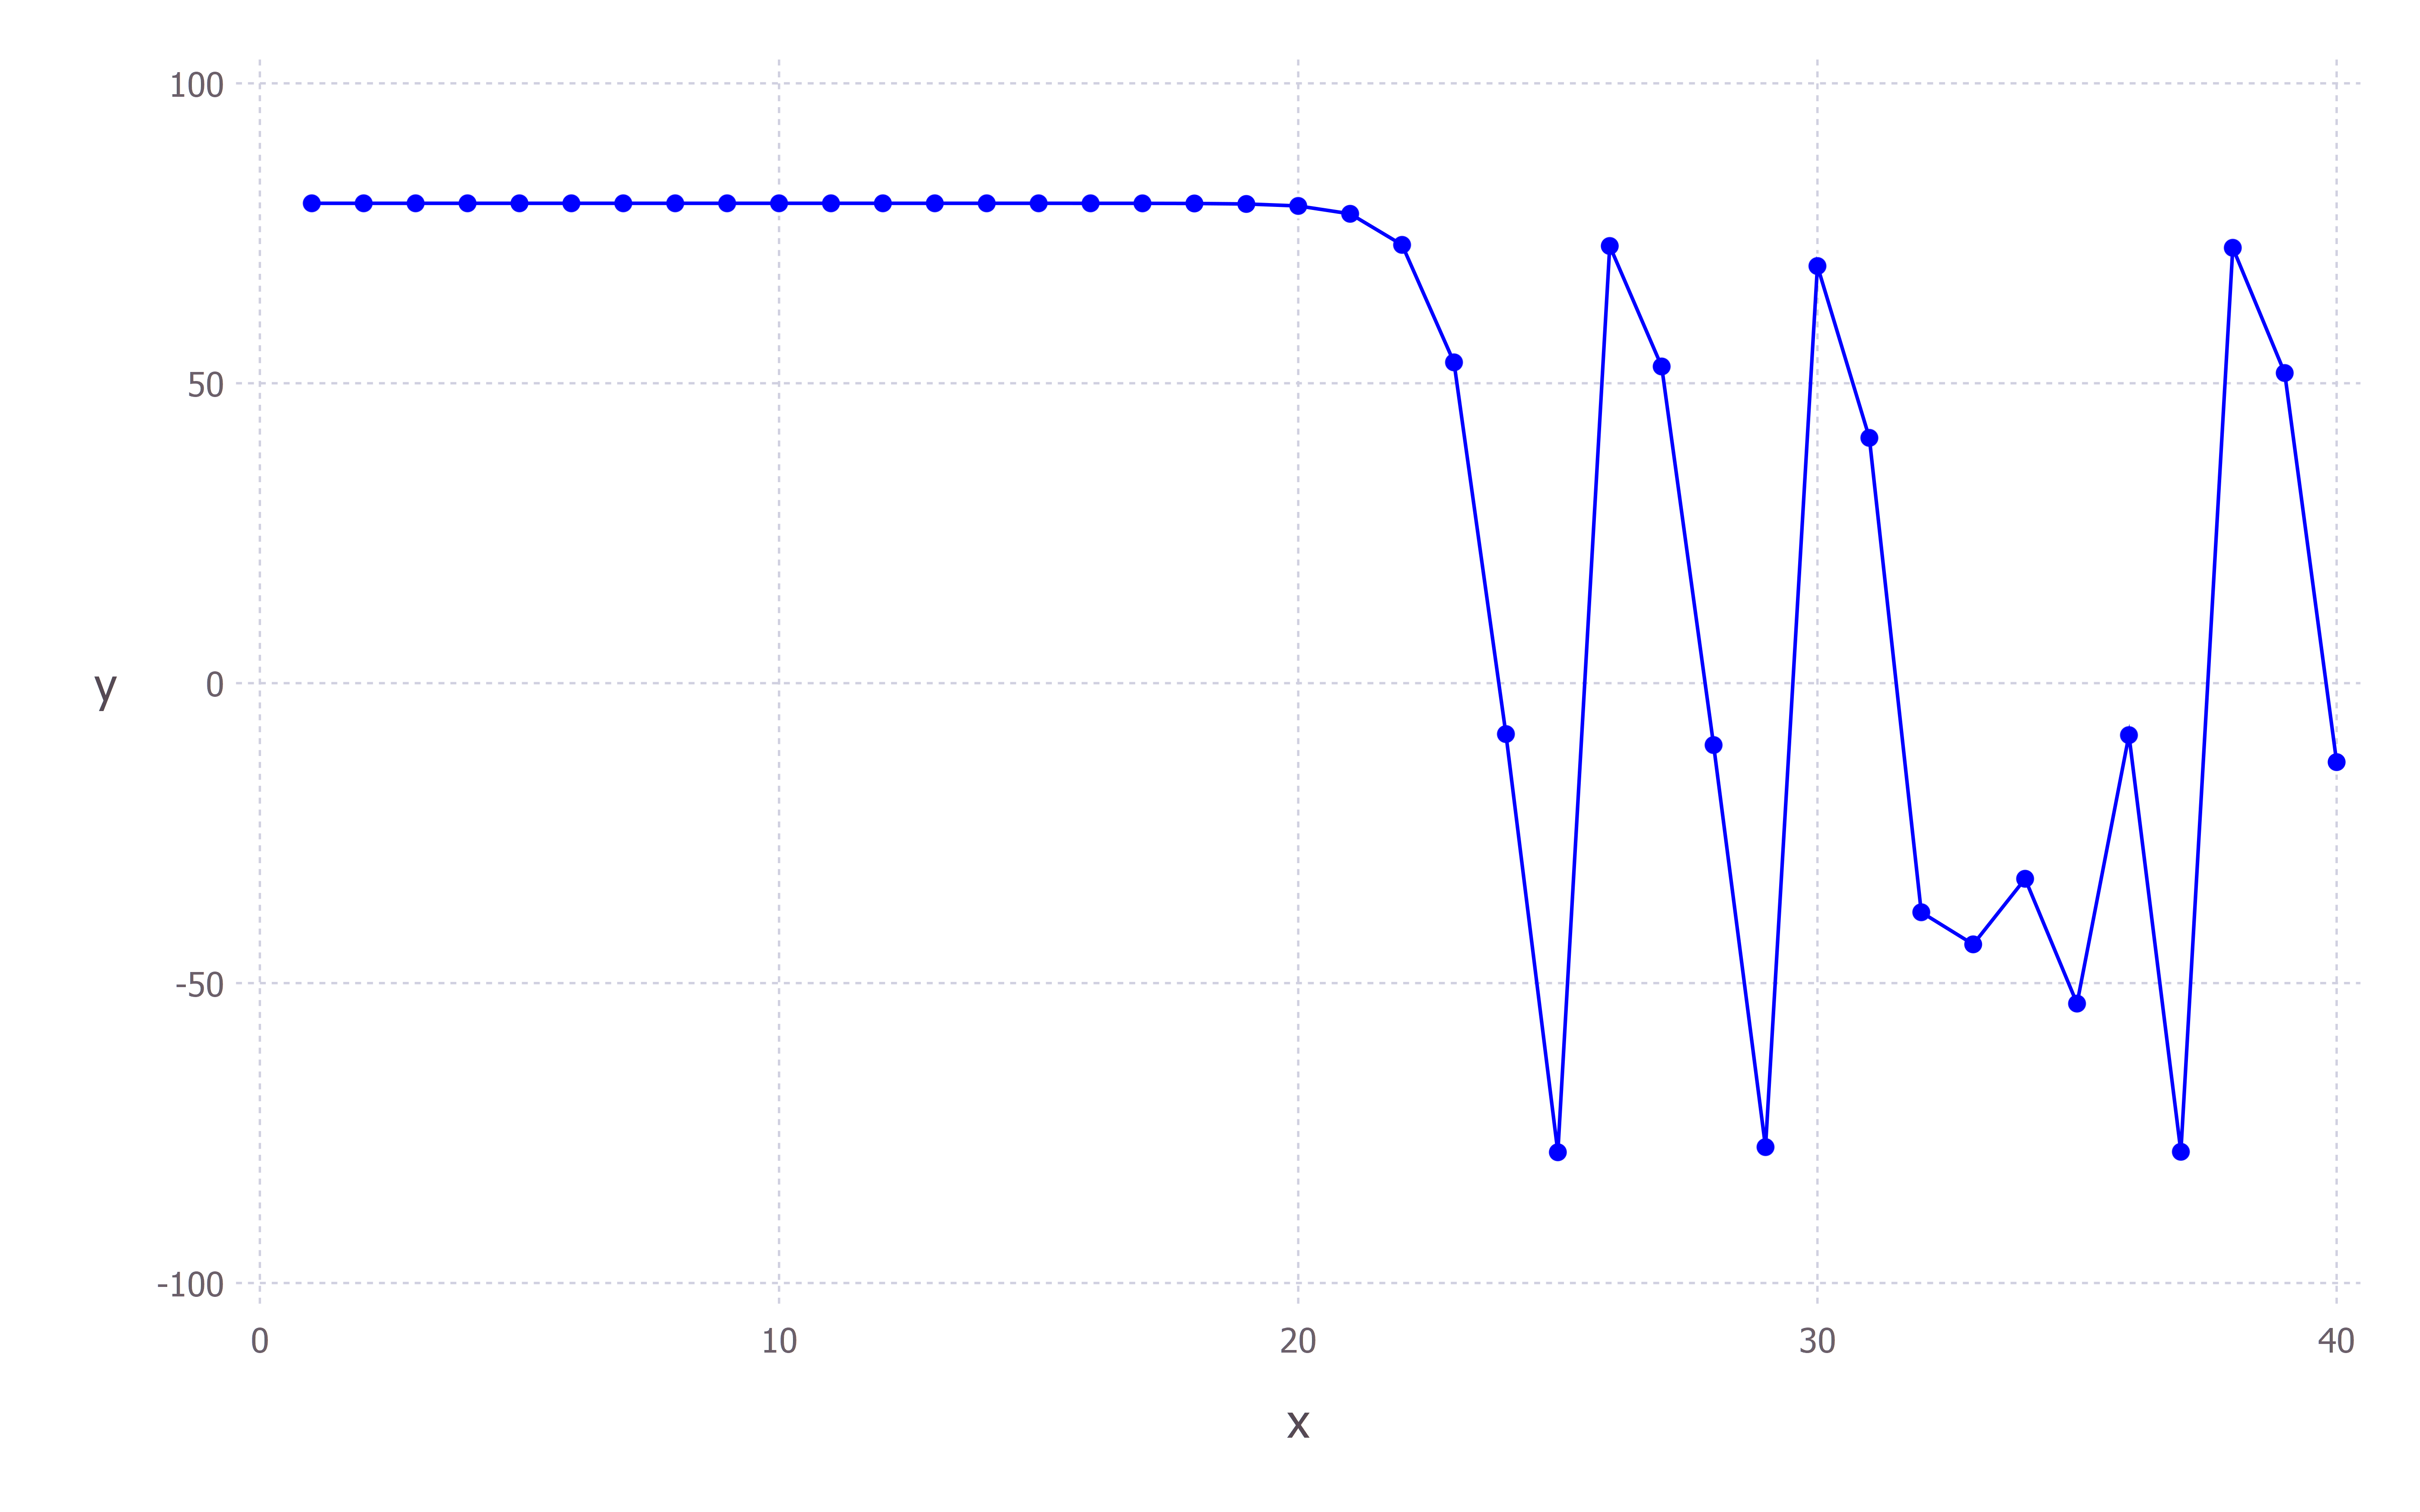
\includegraphics[width=0.5\textwidth]{zad6/plot3.png}} \hfill
%			\subfloat[2.][Plot6]{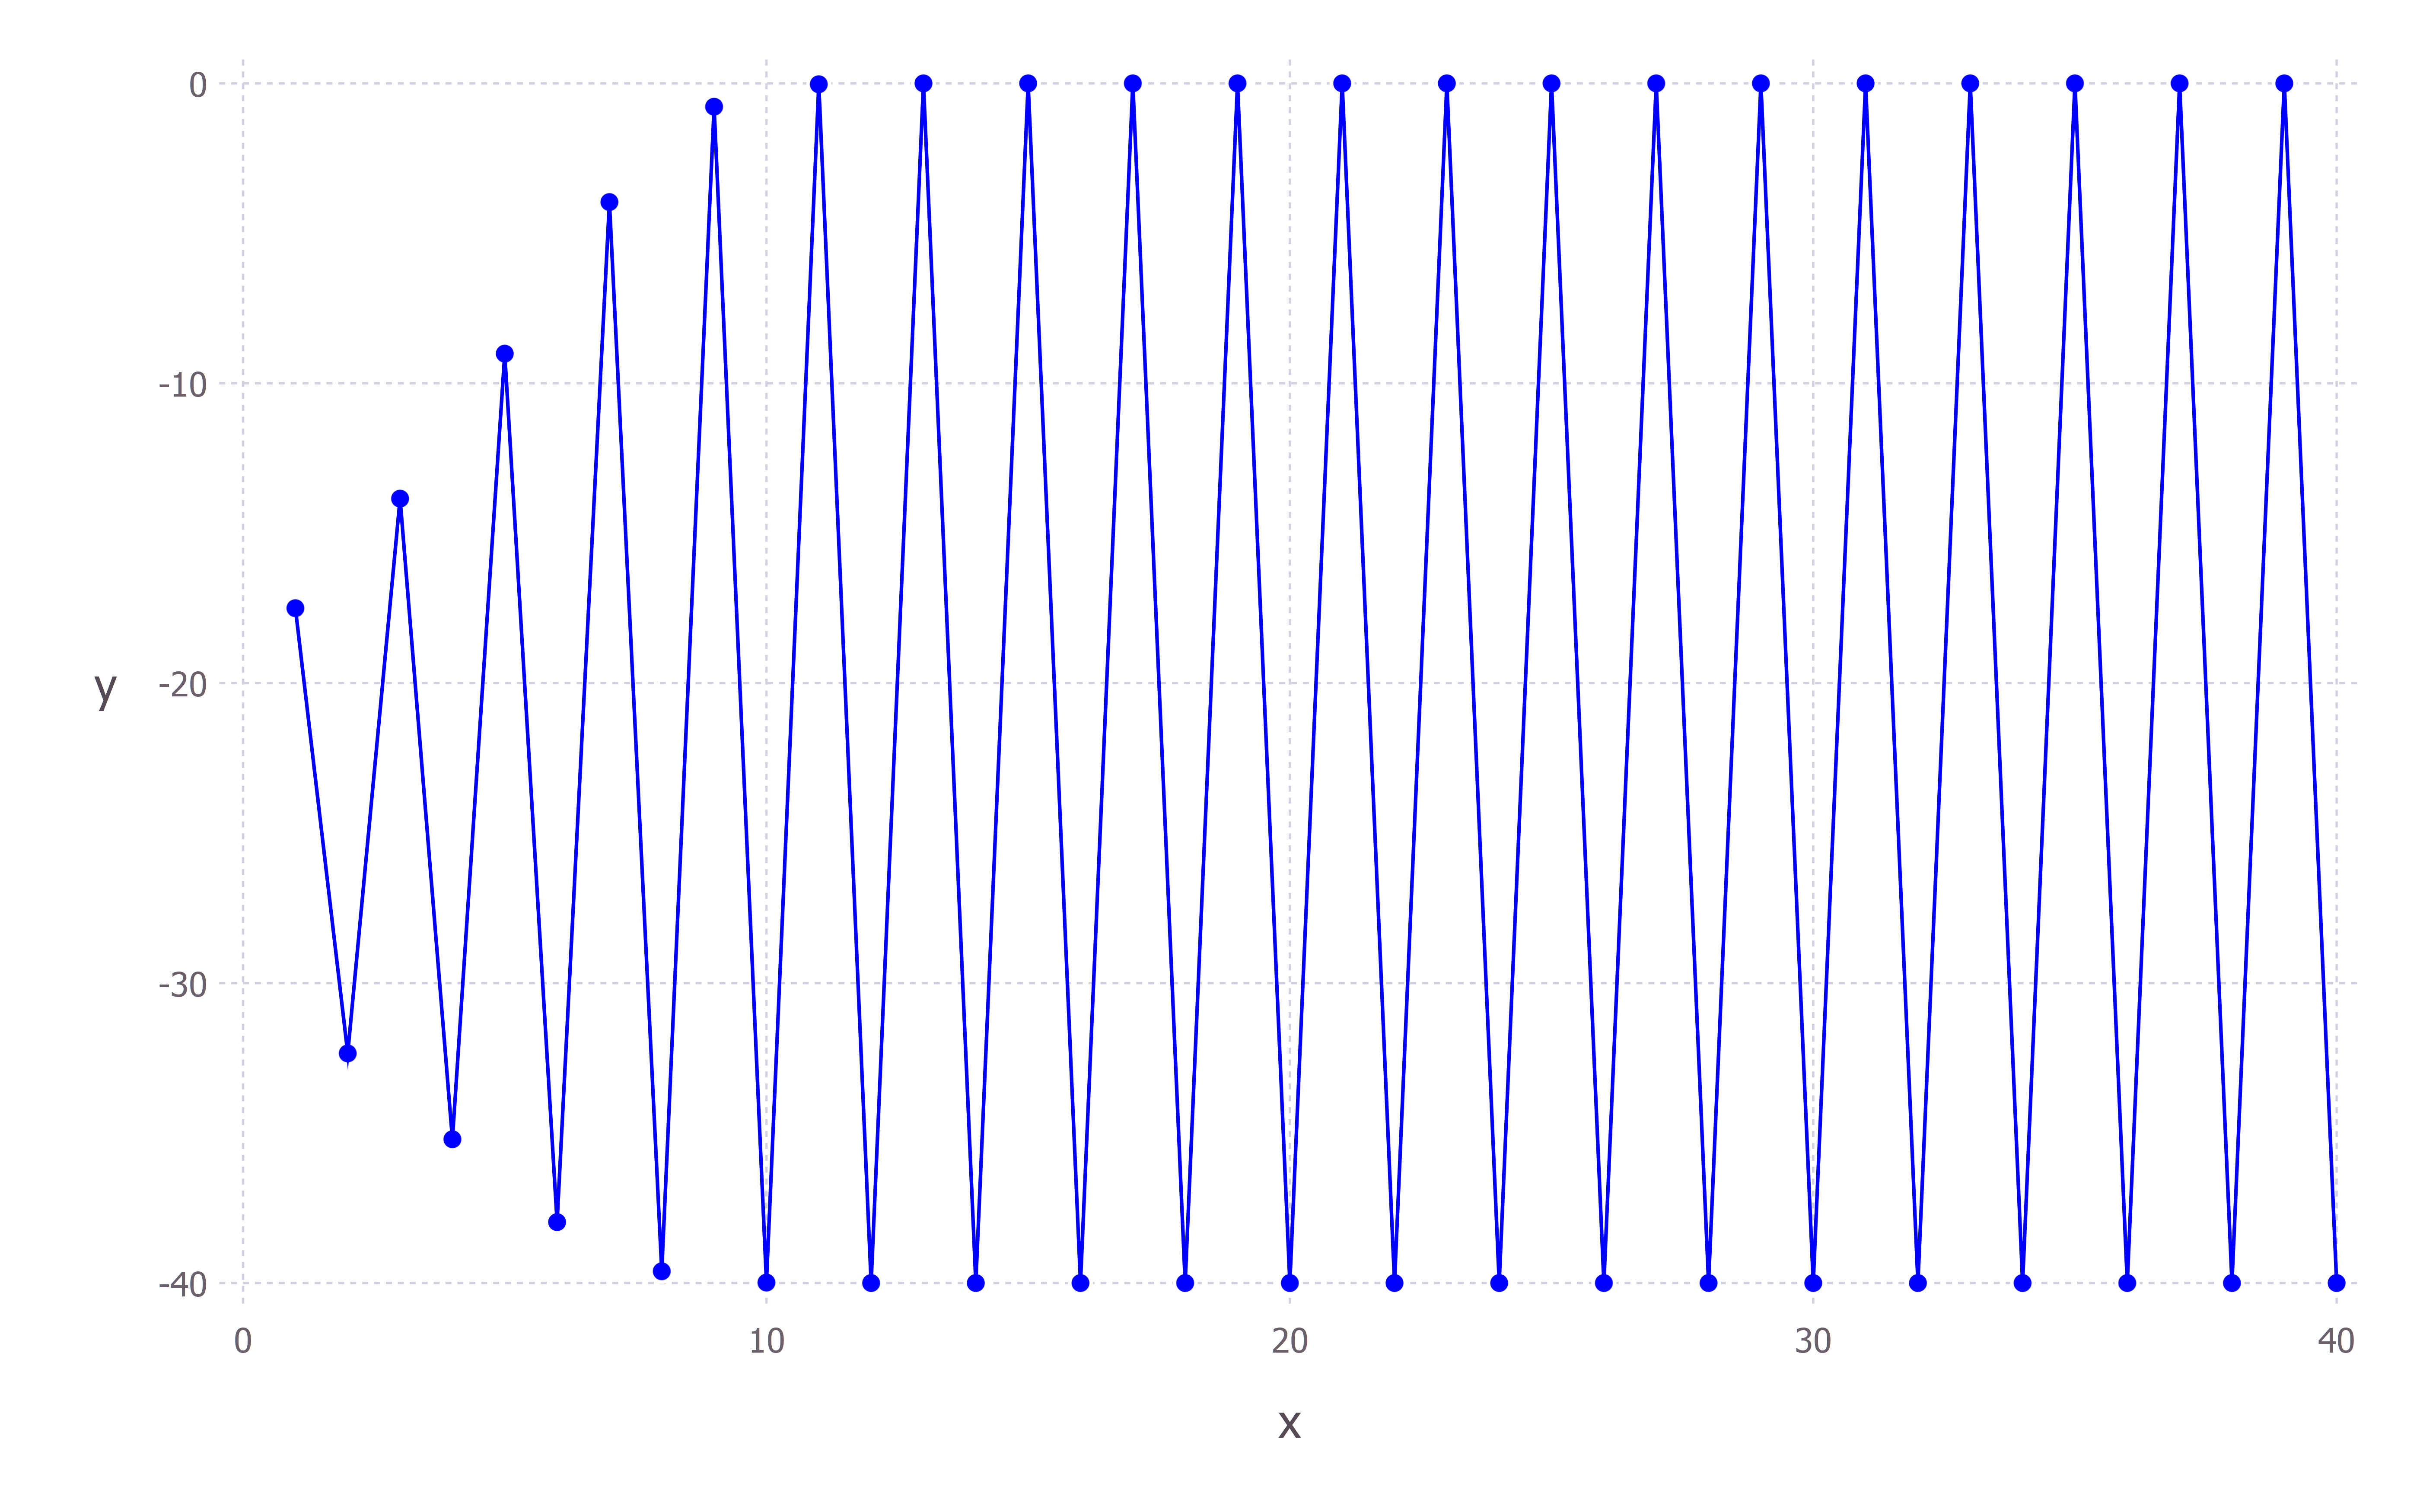
\includegraphics[width=0.5\textwidth]{zad6/plot6.png}} \hfill
%			\subfloat[3.][Plot7]{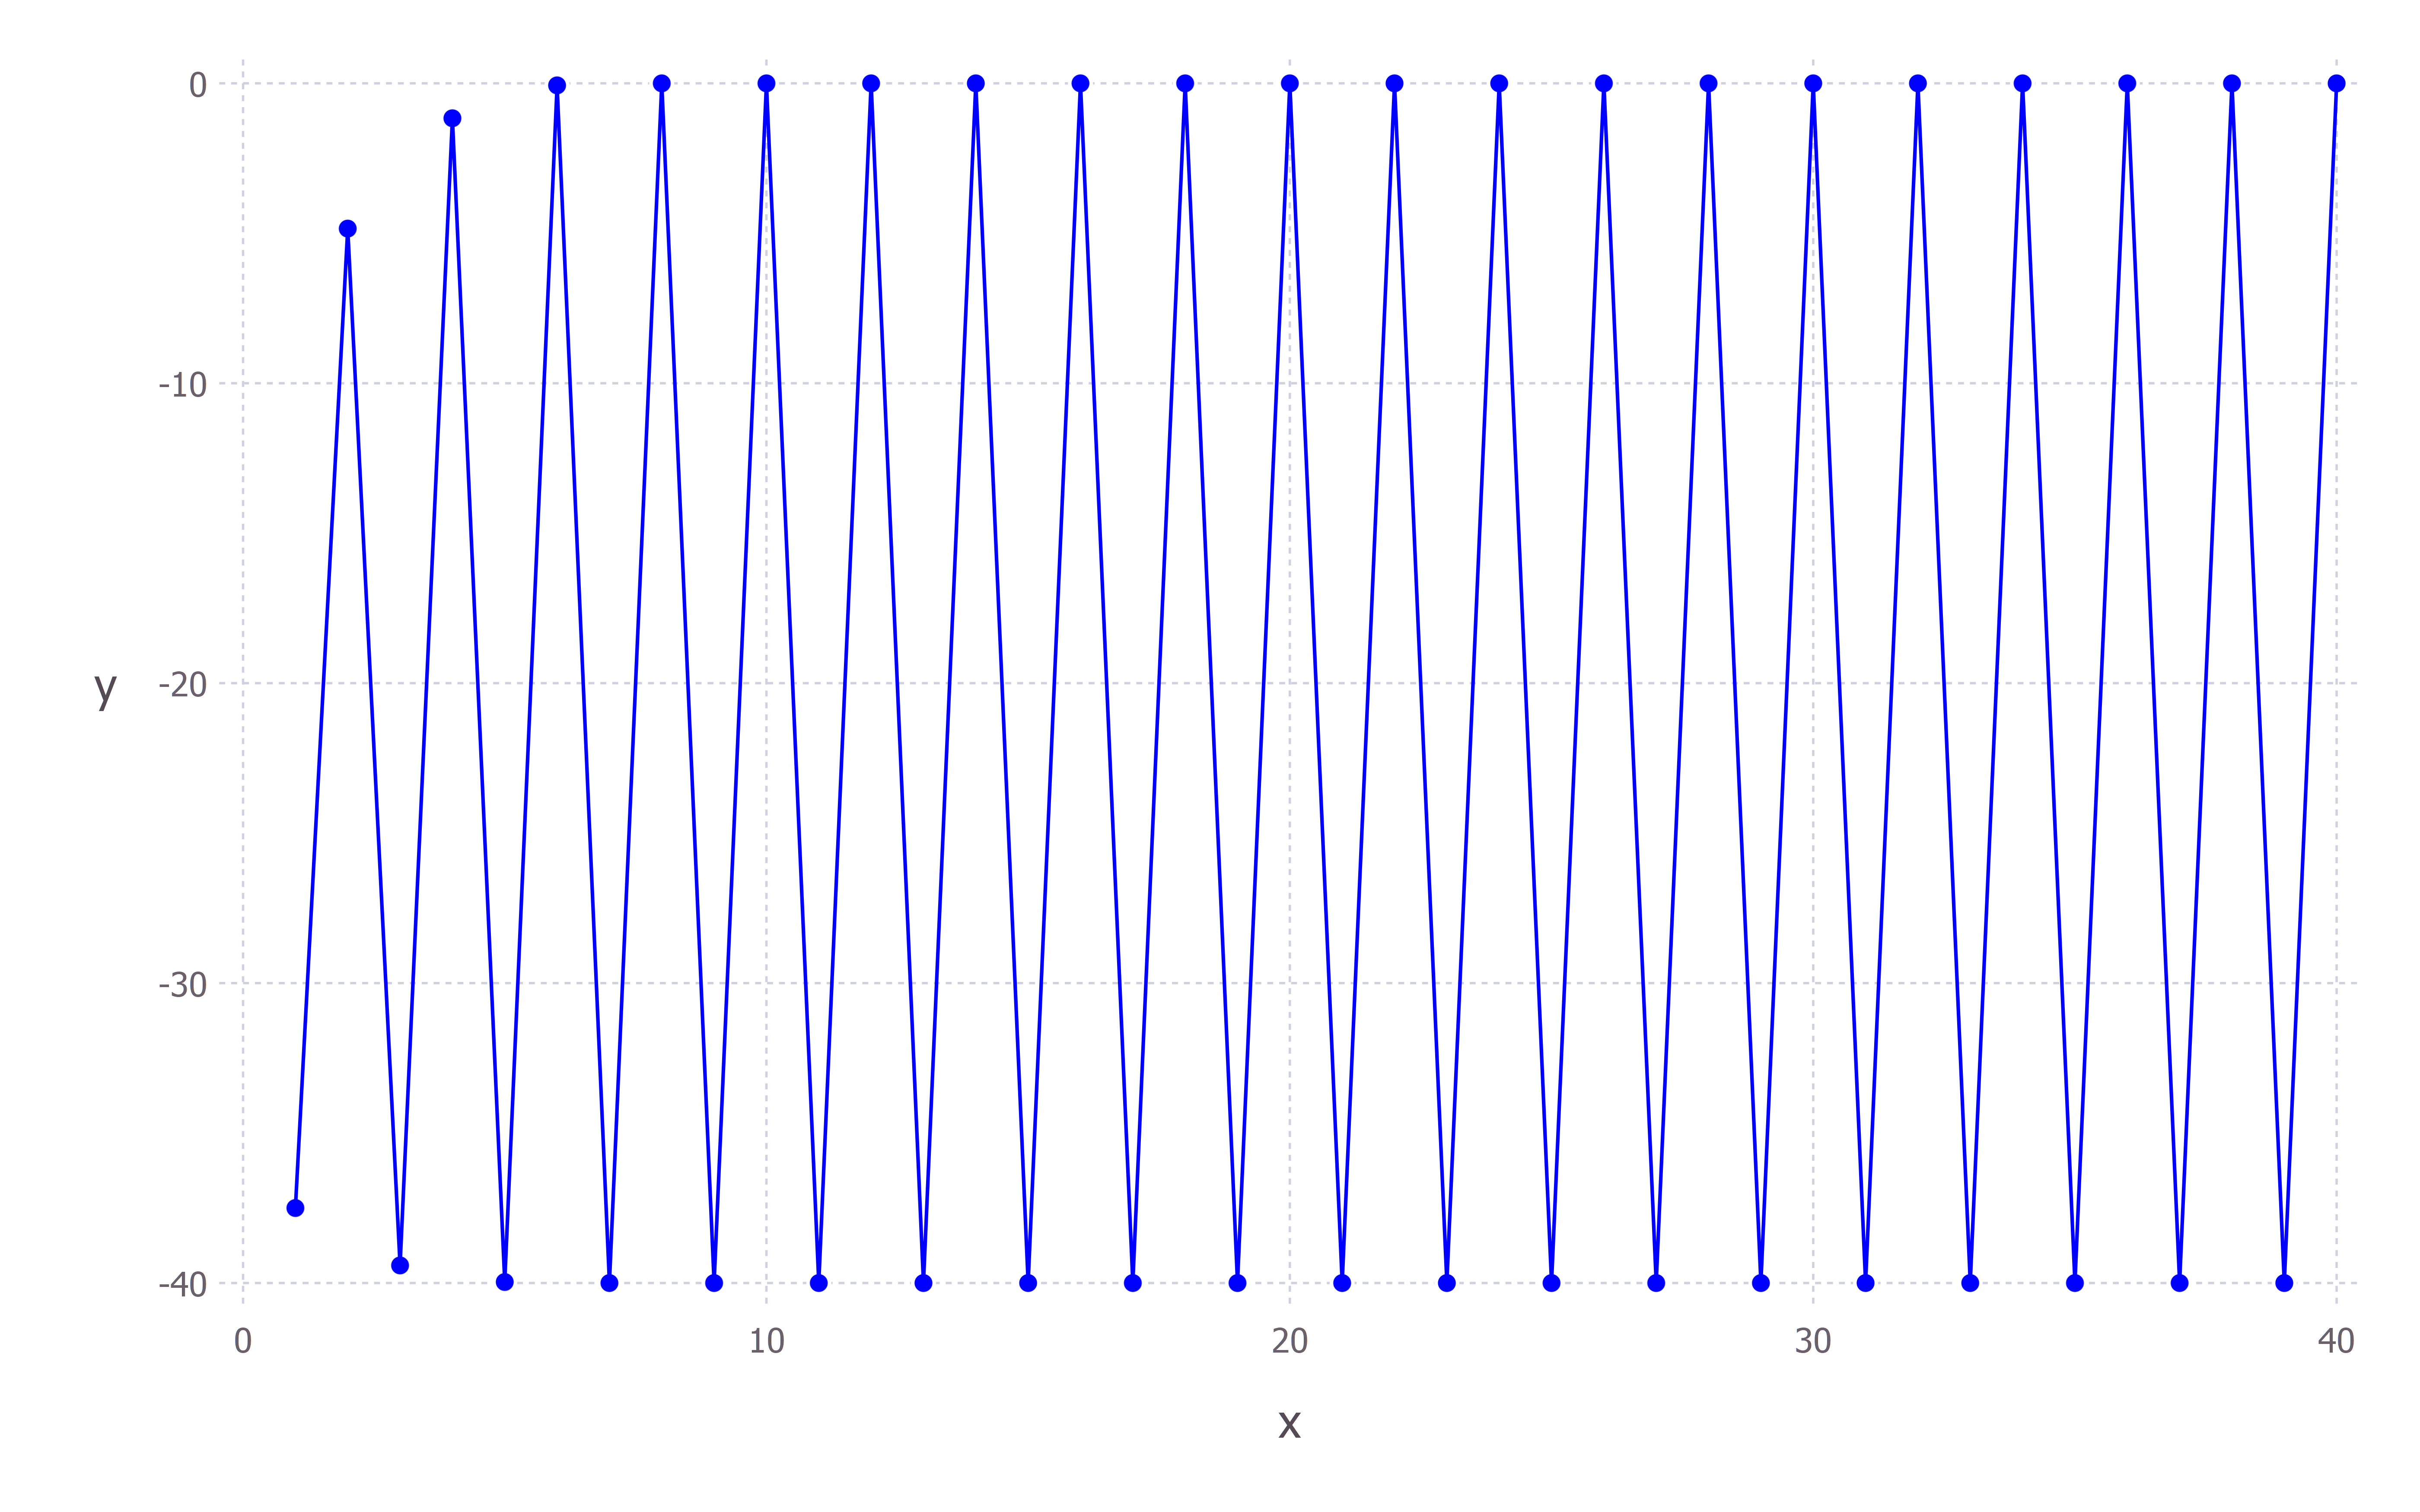
\includegraphics[width=0.5\textwidth]{zad6/plot7.png}}
%  			\caption{Zestawienie wyników dla konkretnych danych}
%  			\label{fig:6}
%		\end{figure}	
